\section{Évaluation de l'hypothèse sur les coûts}
\label{section:4.3-HYPOTHESE-COUTS}
% : « \textit{combien dois-je investir ?} »

	%%% Formulation des hypothèses:
	Pour compléter l'étude réalisée sur l'hypothèse d'efficience (optimisation des paramètres de convergence, cf. section~\ref{section:4.2-HYPOTHESE-EFFICIENCE}), nous aimerions vérifier l'hypothèse suivante :
	\todo{à compléter}

	\begin{tcolorbox}[
		title=\faVial~\textbf{Hypothèse sur les coûts}~\faVial,
		colback=colorTcolorboxHypothesis!15,
		colframe=colorTcolorboxHypothesis!75,
		width=\linewidth
	]
		% Hypothèse.
		«\textbf{
			Il est possible d'\textbf{estimer les coûts nécessaires} d'une méthodologie d'annotation basée sur le \textit{clustering} interactif pour obtenir une base d'apprentissage exploitable. Nous étudierons en particulier les coûts relatifs au temps d'annotation, au temps de calculs des algorithmes, ainsi que la durée totale de la méthode en fonction de la taille du jeu de données.
		} » \\

		% Résumé des études.
		Afin de vérifier cette hypothèse, nous organiserons plusieurs expériences pour simuler ou déterminer ces durées : une étude du temps d'annotation par un expert métier (cf. section~\ref{section:4.3.1-ETUDE-COUTS-TEMPS-ANNOTATION}), une étude du temps de calcul des algorithmes (cf. section~\ref{section:4.3.2-ETUDE-COUTS-TEMPS-CALCUL}) et une étude du nombre de contraintes nécessaires (cf. section~\ref{section:4.3.3-ETUDE-COUT-NOMBRE-CONTRAINTES}). Nous conclurons l'estimation du temps total d'un projet d'annotation en section~\ref{section:4.3.4-ETUDE-COUTS-TOTAL}.
		
		% Figure.
		La figure~\ref{figure:4.3-HYPOTHESE-COUTS} illustre cette hypothèse et l'espoir de pouvoir caractériser la qualité de la base d'apprentissage en cours de construction en fonction d'un coût temporel au lieu d'un nombre abstrait d'itérations de la méthode. 
		%
		
		\begin{figure}[H]  % keep [H] to be in the tcolorbox.
			\centering
			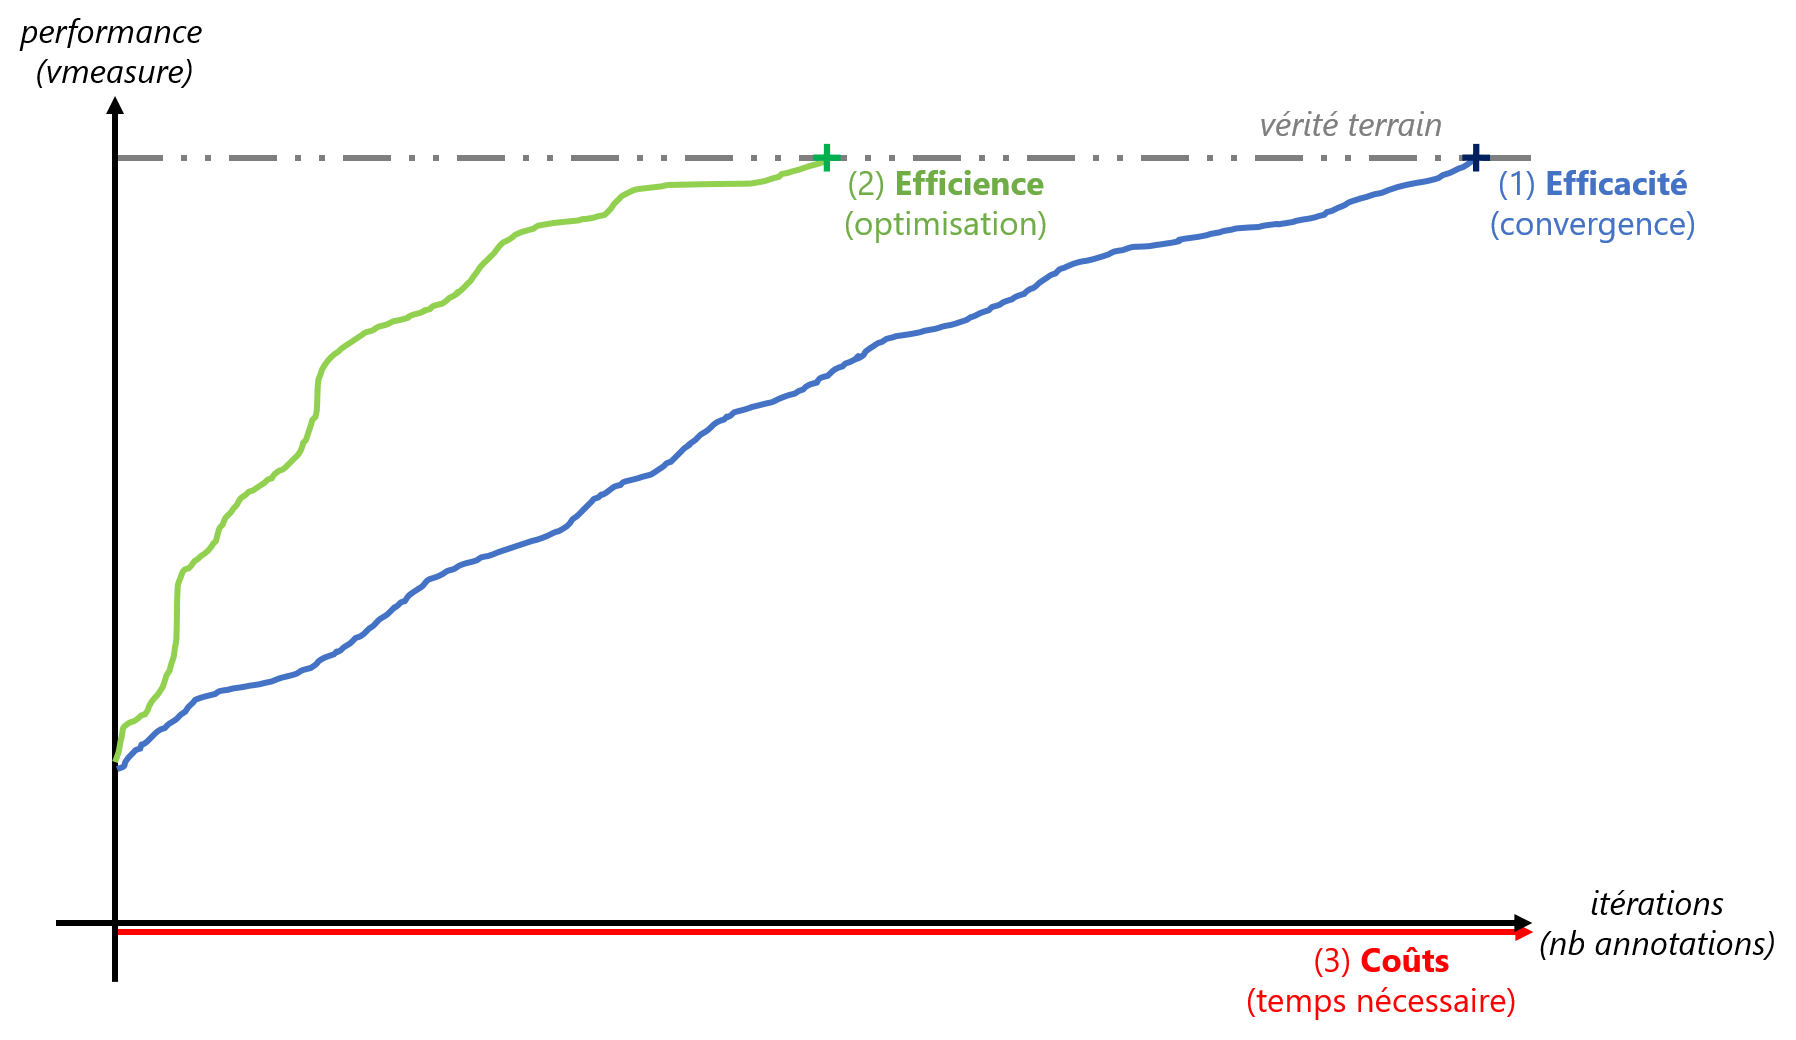
\includegraphics[width=0.8\textwidth]{figures/hypotheses-03-couts}
			\caption{Illustration des études réalisées sur le \textit{clustering} interactif (\textit{étape 3/6}) en schématisant l'évolution de la performance (\textit{accord avec la vérité terrain calculé en v-measure}) d'une base d'apprentissage en cours de construction en fonction du nombre d'itérations de la méthode (\textit{nombre d'annotations par un expert métier}).}
			\label{figure:4.3-HYPOTHESE-COUTS}
		\end{figure}

	\end{tcolorbox}
	
	
	%%%
	%%% Subsection 4.3.1: Étude du temps d'annotation nécessaire pour traiter un lot de contraintes en chronométrant des opérateurs en situation réelle
	%%%
	\subsection{Étude du temps d'annotation nécessaire pour traiter un lot de contraintes en chronométrant des opérateurs en situation réelle}
	\label{section:4.3.1-ETUDE-COUTS-TEMPS-ANNOTATION}
	
		%%% Protocole expérimental.
		\subsubsection{Protocole expérimental}
		
			% Objectif de l'expérience.
			Nous voulons estimer le temps nécessaire à un opérateur pour annoter un lot de contraintes.
			Pour cela, nous allons chronométrer plusieurs expert métiers en train d'annoter un même échantillon et modéliser le nombre de contraintes par minute ainsi que son évolution au cours de plusieurs sessions d'annotation.
			
			% Axiome.
			\begin{leftBarWarning}
				Dans cette étude, nous supposons que les annotateurs de l'expérience connaissent parfaitement le domaine traité dans le jeu de données, et qu'ils sont capables de caractériser sans ambiguïté la similitude entre deux données issues de cet ensemble.
				Afin de pourvoir faire cette hypothèse forte, et ainsi limiter les bruits dans l'analyse des résultats, le jeu de données devra traiter d'un sujet de culture générale (ne nécessitant donc pas de connaissance particulière) et des réviseurs devront supprimer en amont et d'un commun accord les données trop spécifiques.
			\end{leftBarWarning}
			
			% Pseudo-code.
			Pour résumer le protocole expérimental que nous décrivons ci-dessous, vous pouvez vous référer au pseudo-code décrit dans Alg.~\ref{algorithm:4.3.1-ETUDE-COUTS-TEMPS-ANNOTATION-PROTOCOLE}.
			%
			\begin{algorithm}[!htb]
				\begin{algorithmic}[1]
					\Require jeu de données annoté (vérité terrain)
					\Require plusieurs réviseurs, plusieurs annotateurs
					\State \textbf{initialisation} définir et revoir le jeu de données entre réviseurs
					\State \textbf{échantillonnage} sélectionner une base de contraintes avec \texttt{samp.rand.full}
					\ForAll{annotateur}
						\While{la base de contraintes n'a pas été entièrement annotée}
							\State \textbf{chronomètre: START}
							\State \textbf{annotation}: annoter une partie des contraintes
							\State \textbf{revue}: revue des contraintes en conflits d'annotation
							\State \textbf{chronomètre: STOP}
							\State \textbf{mesure}: estimer la différence de chronomètre pour cette session
						\EndWhile
					\EndFor
					\State \textbf{modélisation}: entraîner un modèle linéaire généralisé du temps d'annotation
					\State \textbf{simulation}: écrire l'équation du temps d'annotation d'un lot de contraintes
					\Ensure modélisation du temps d'annotation d'un lot de contraintes
				\end{algorithmic}
				\caption{Description en pseudo-code du protocole expérimental de l'étude du temps d'annotation d'un lot de contraintes par un expert métier.}
				\label{algorithm:4.3.1-ETUDE-COUTS-TEMPS-ANNOTATION-PROTOCOLE}
			\end{algorithm}
			
			% Détails de l'expérience : préparation du jeu de données.
			Pour cette étude, nous procéderons en plusieurs étapes.
			D'abord, il faut choisir un jeu de données approprié : pour valider notre hypothèse forte sur les compétence de nos annotateurs, nous cherchons un jeu de données traitant d'un sujet de culture général.
			Pour cette expérience, nous avons donc choisi une collecte des titres d'articles de journaux classés par catégorie de publication (\textit{économie}, \textit{sport},...).
			Comme certains titres peuvent porter à confusion (un titre d'article n'étant pas toujours explicite sur son contenu), deux réviseurs sont chargés de choisir les données les plus explicites sur un échantillon d'un millier de données représentatives des $14$ catégories les plus communes.
			L'échantillon résultant est décrit en annexe~\todo{TODO: ANNEXE JEU DE DONNEES}.
			
			% Détails de l'expérience : sélection des contraintes à annoter. 
			A partir de ces données, nous sélectionnons un lot de $1~000$ contraintes à annoter. Comme nous nous intéressons exclusivement au temps d'annotation pour cette expérience (et que nous ne regardons pas le nombre d'itérations de la méthode), nous utilisons l'échantillonnage purement aléatoire (\texttt{samp.rand.full}).			
			
			% Détails de l'expérience : annotations et consignes.
			Ensuite, un groupe de $14$ annotateurs vont annoter la sélection de $1~000$ contraintes en plusieurs sessions.
			Les directives données aux opérateurs sont les suivantes:
			\begin{itemize}
				\item \textbf{Contexte de l'opérateur} :
				« \textit{Vous êtes des \textbf{experts de la presse et de l’actualité} ; Vous voulez classer des articles dans des catégories en fonction de leur titre ; Vous ne savez pas précisément quelles catégories vous allez utiliser pour classer vos articles ; Mais vous savez \textbf{caractériser la similitude} de deux articles} » ;
				\item \textbf{Contexte sur le jeu de données} :
				« \textit{Le thème sont les catégories d’articles de presse ; La vérité terrain contient entre 10 et 20 catégories parmi les plus communes de la presse ; La vérité terrain contient entre 30 et 100 articles par catégorie ; Vous \textbf{pouvez regarder le jeu de données non annoté} autant que vous le voulez} » ;
				\item \textbf{Objectif de l'expérience} :
				« \textit{Je veux savoir le temps nécessaire pour annoter un certain nombre de contraintes ; Autrement dit : \textbf{Pour annoter 1000 contraintes, combien de temps me faut-il ?}} » ;
				\item \textbf{Consignes d'annotations} :
				« \textit{Faites des séries de \textbf{15 minutes minimum} pour avoir de la régularité ; Si possible, \textbf{isolez-vous} pour ne pas être dérangé et ne pas fausser les résultats ; Pour chaque série, \textbf{notez le temps et le nombre de contraintes annotés} ; Si vous ne savez pas quoi annoter (trop ambigu, vocabulaire inconnu, ...), \textbf{passez au suivant sans annoter} (vous êtes sensés être des experts de la presse !)} ».
			\end{itemize}
			%
			Pour réaliser l'annotation, les opérateurs auront accès à l'application web développée au cours de ce doctorat.
			Des captures d'écran sont disponibles en figures~\ref{figure:4.3.1-ETUDE-COUTS-TEMPS-ANNOTATION-APPLICATION-ANNOTATION}et~\ref{figure:4.3.1-ETUDE-COUTS-TEMPS-ANNOTATION-APPLICATION-LISTE-CONTRAINTES}.
			Une description plus détaillée de l'application et de ses fonctionnalités est disponible en section~\ref{section:3.3-DESCRIPTION-IMPLEMENTATION}\todo{description à faire}
			%
			\begin{figure}[!htb]
				\centering
				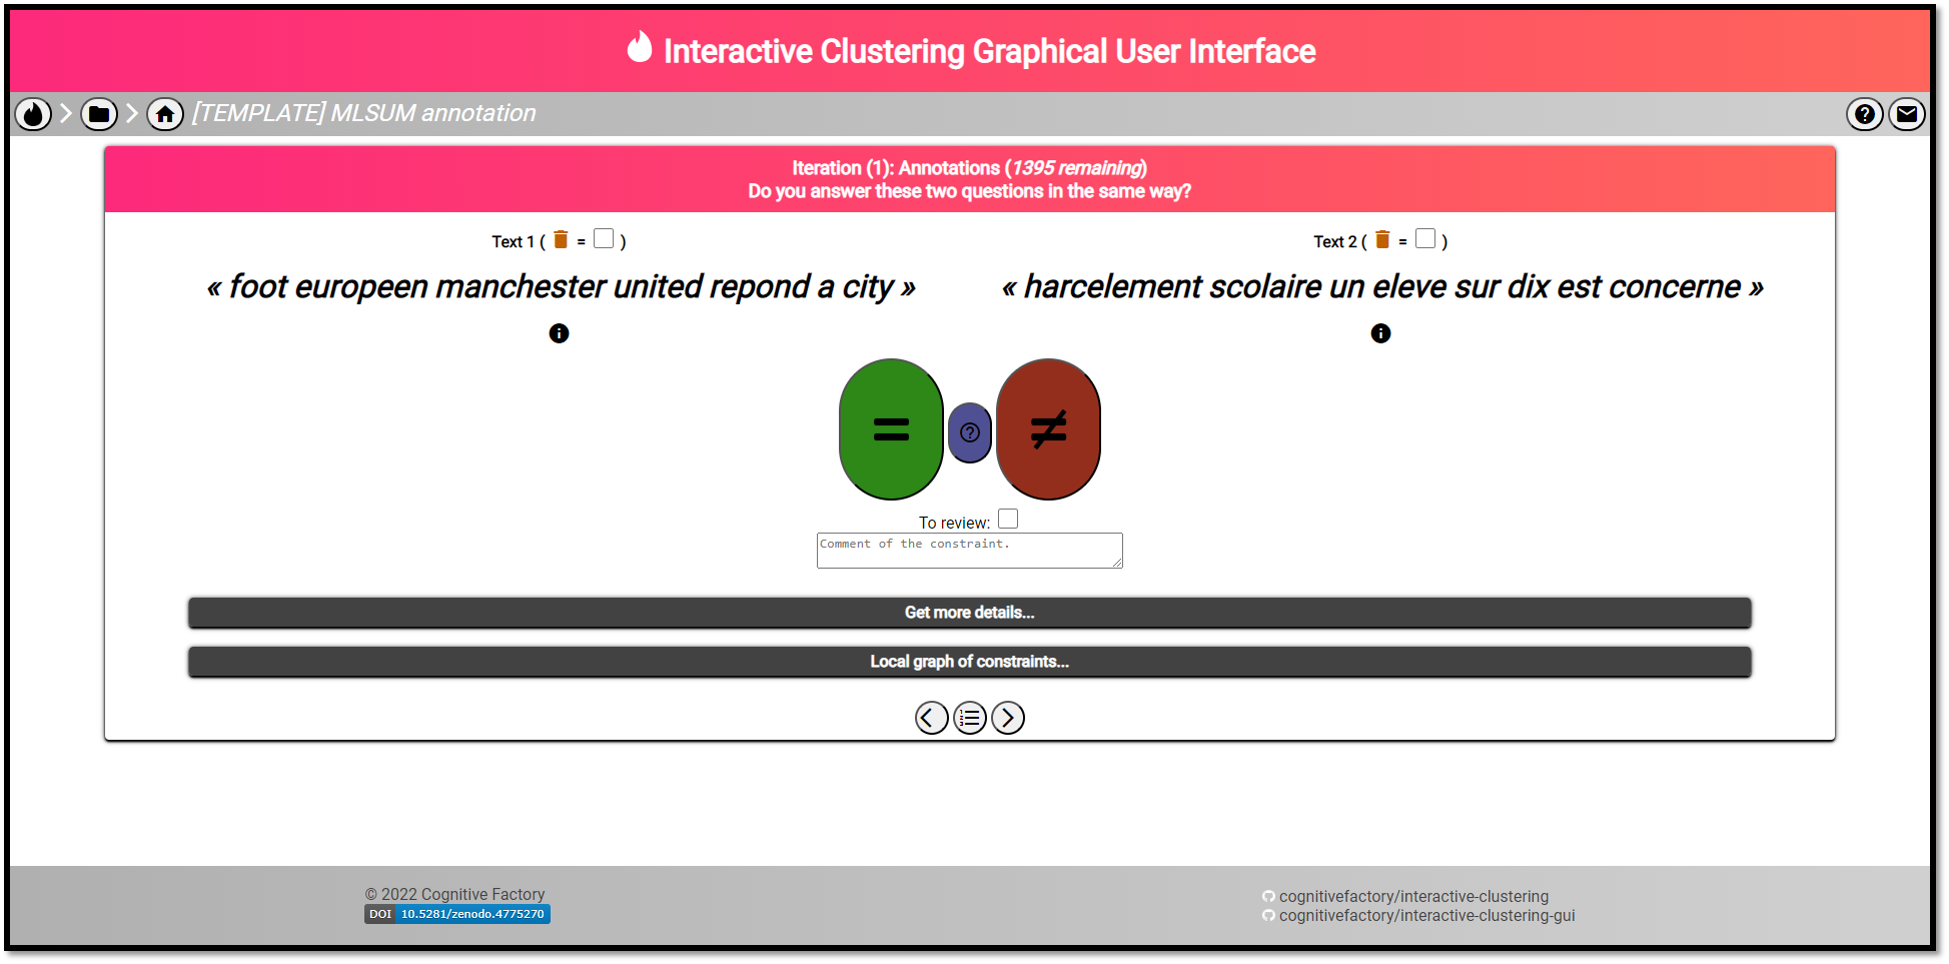
\includegraphics[width=\textwidth]{figures/etude-temps-annotation-0application-annotation}
				\caption{Capture d'écran de l'application web permettant utilisant notre méthodologie de \textit{clustering} interactif pour annoter des contraintes (page d'annotation)}
				\label{figure:4.3.1-ETUDE-COUTS-TEMPS-ANNOTATION-APPLICATION-ANNOTATION}
			\end{figure}
			\begin{figure}[!htb]
				\centering
				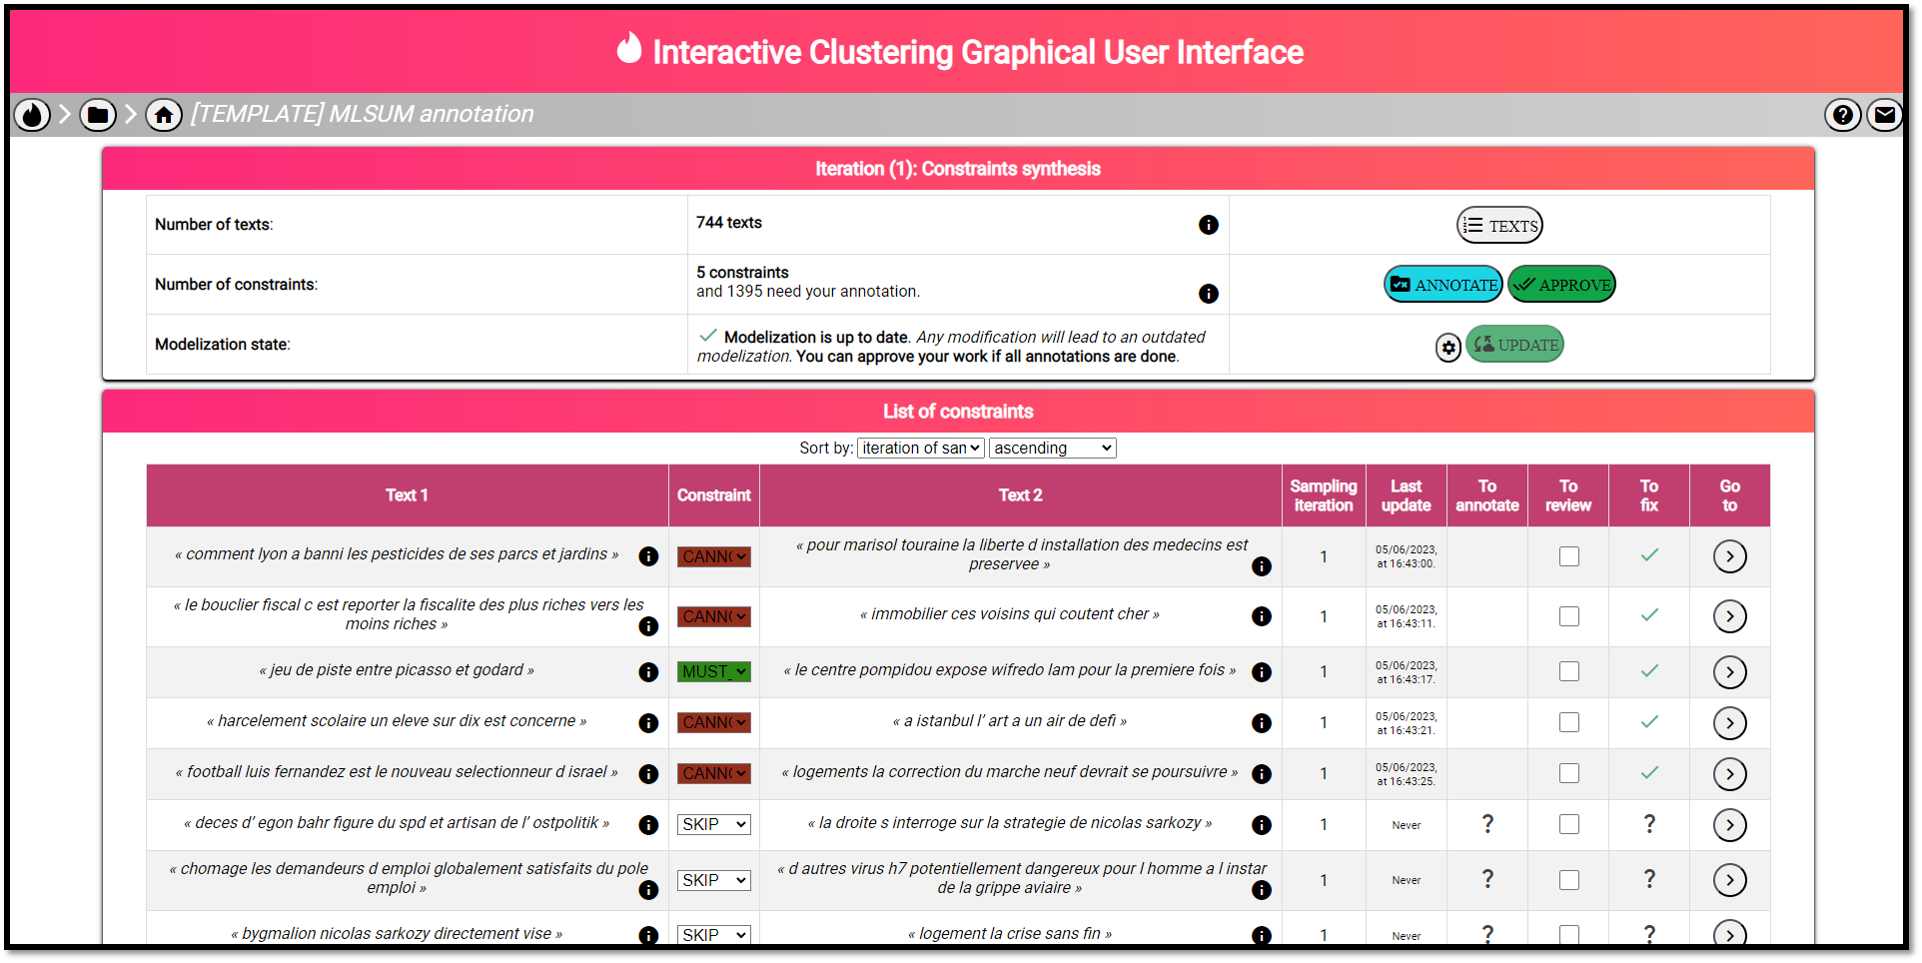
\includegraphics[width=\textwidth]{figures/etude-temps-annotation-0application-liste-contraintes}
				\caption{Capture d'écran de l'application web permettant utilisant notre méthodologie de \textit{clustering} interactif pour annoter des contraintes (page d'inventaire des contraintes à annoter)}
				\label{figure:4.3.1-ETUDE-COUTS-TEMPS-ANNOTATION-APPLICATION-LISTE-CONTRAINTES}
			\end{figure}
			
			
			% Détails de l'expérience : modélisation.
			Une fois les sessions d'annotations terminées, nous entraînons un modèle linéaire généralisé (\textit{GLM}) pour estimer le temps d'annotation moyen pour un lot de contraintes. Ce modèle sera caractérisé par le coefficient de détermination généralisé \texttt{R²} de \textit{Cox et Snel}, la log-vraisemblance \texttt{llf} et la log-vraisemblance \texttt{llf\_null} du modèle \textit{null}.
			Nous discuterons aussi de l'évolution de la vitesse d'un opérateur au cours des différentes sessions d'annotation.

			% Référence scripts.
			\begin{leftBarInformation}
				Ces analyses sont réalisées en Python à l'aide des librairies \texttt{datetime} et \texttt{statsmodels} (\cite{seabold:2010}).
				Le projet à importer dans l'outil d'annotation ainsi que les scripts de l'expérience (\textit{notebooks} Python) sont disponibles dans un dossier dédié de~\cite{schild:cognitivefactory-interactive-clustering-comparative-study:2021}.
			\end{leftBarInformation}
			\todo{citation}

		%%% Résultats
		\subsubsection{Résultats obtenus}
		
			% Taux de participation.
			Durant cette expérience, $14$ annotateurs ont participé à l'annotation de $1~000$ contraintes aléatoires sur un jeu de données.
			Par manque de disponibilités, $4$ annotateurs n'ont que partiellement réalisé leur tâche : nous avons toutefois intégré leurs participations car elles contenaient toutes au moins $150$ annotations.
			
			% Statistiques descriptives.
			D'après les observations, un annotateur réalisait en moyenne $170.70$ contraintes par session d'annotation (min: $43$, max: $547$, médiane: $138$, écart-type: $106.37$) ce qui lui demandait en moyenne $23.05$ minutes (min: $3.00$, max: $92.00$, écart-type: $14.41$).
			De plus, la vitesse d'annotation moyenne était de $7.74$ contraintes par minute (min: $3.46$, max: $14.33$, écart-type: $2.93$).
			
			% Modélisation du temps d'annotation.
			Le modèle linéaire généralisé entraîné sur les mesures de temps d'annotations (\texttt{R²}: $0.922$, \texttt{llf}: $-497.37$, \texttt{llf\_null}: $-539.95$) nous permet de déduire l'équation suivante :
			%
			\begin{equation}
				time.annotation~(secondes)~
				\simeq~202 + 6.92 \cdot \texttt{constraints\_number}
			\end{equation}
		
			% Affichage du temps d'annotation.
			La figure~\ref{figure:4.3.1-ETUDE-COUTS-TEMPS-ANNOTATION-SIMULATION} représente cette modélisation du temps d'annotation en comparaison avec les mesures réalisées lors de l'expérience.
			\begin{figure}[!htb]
				\centering
				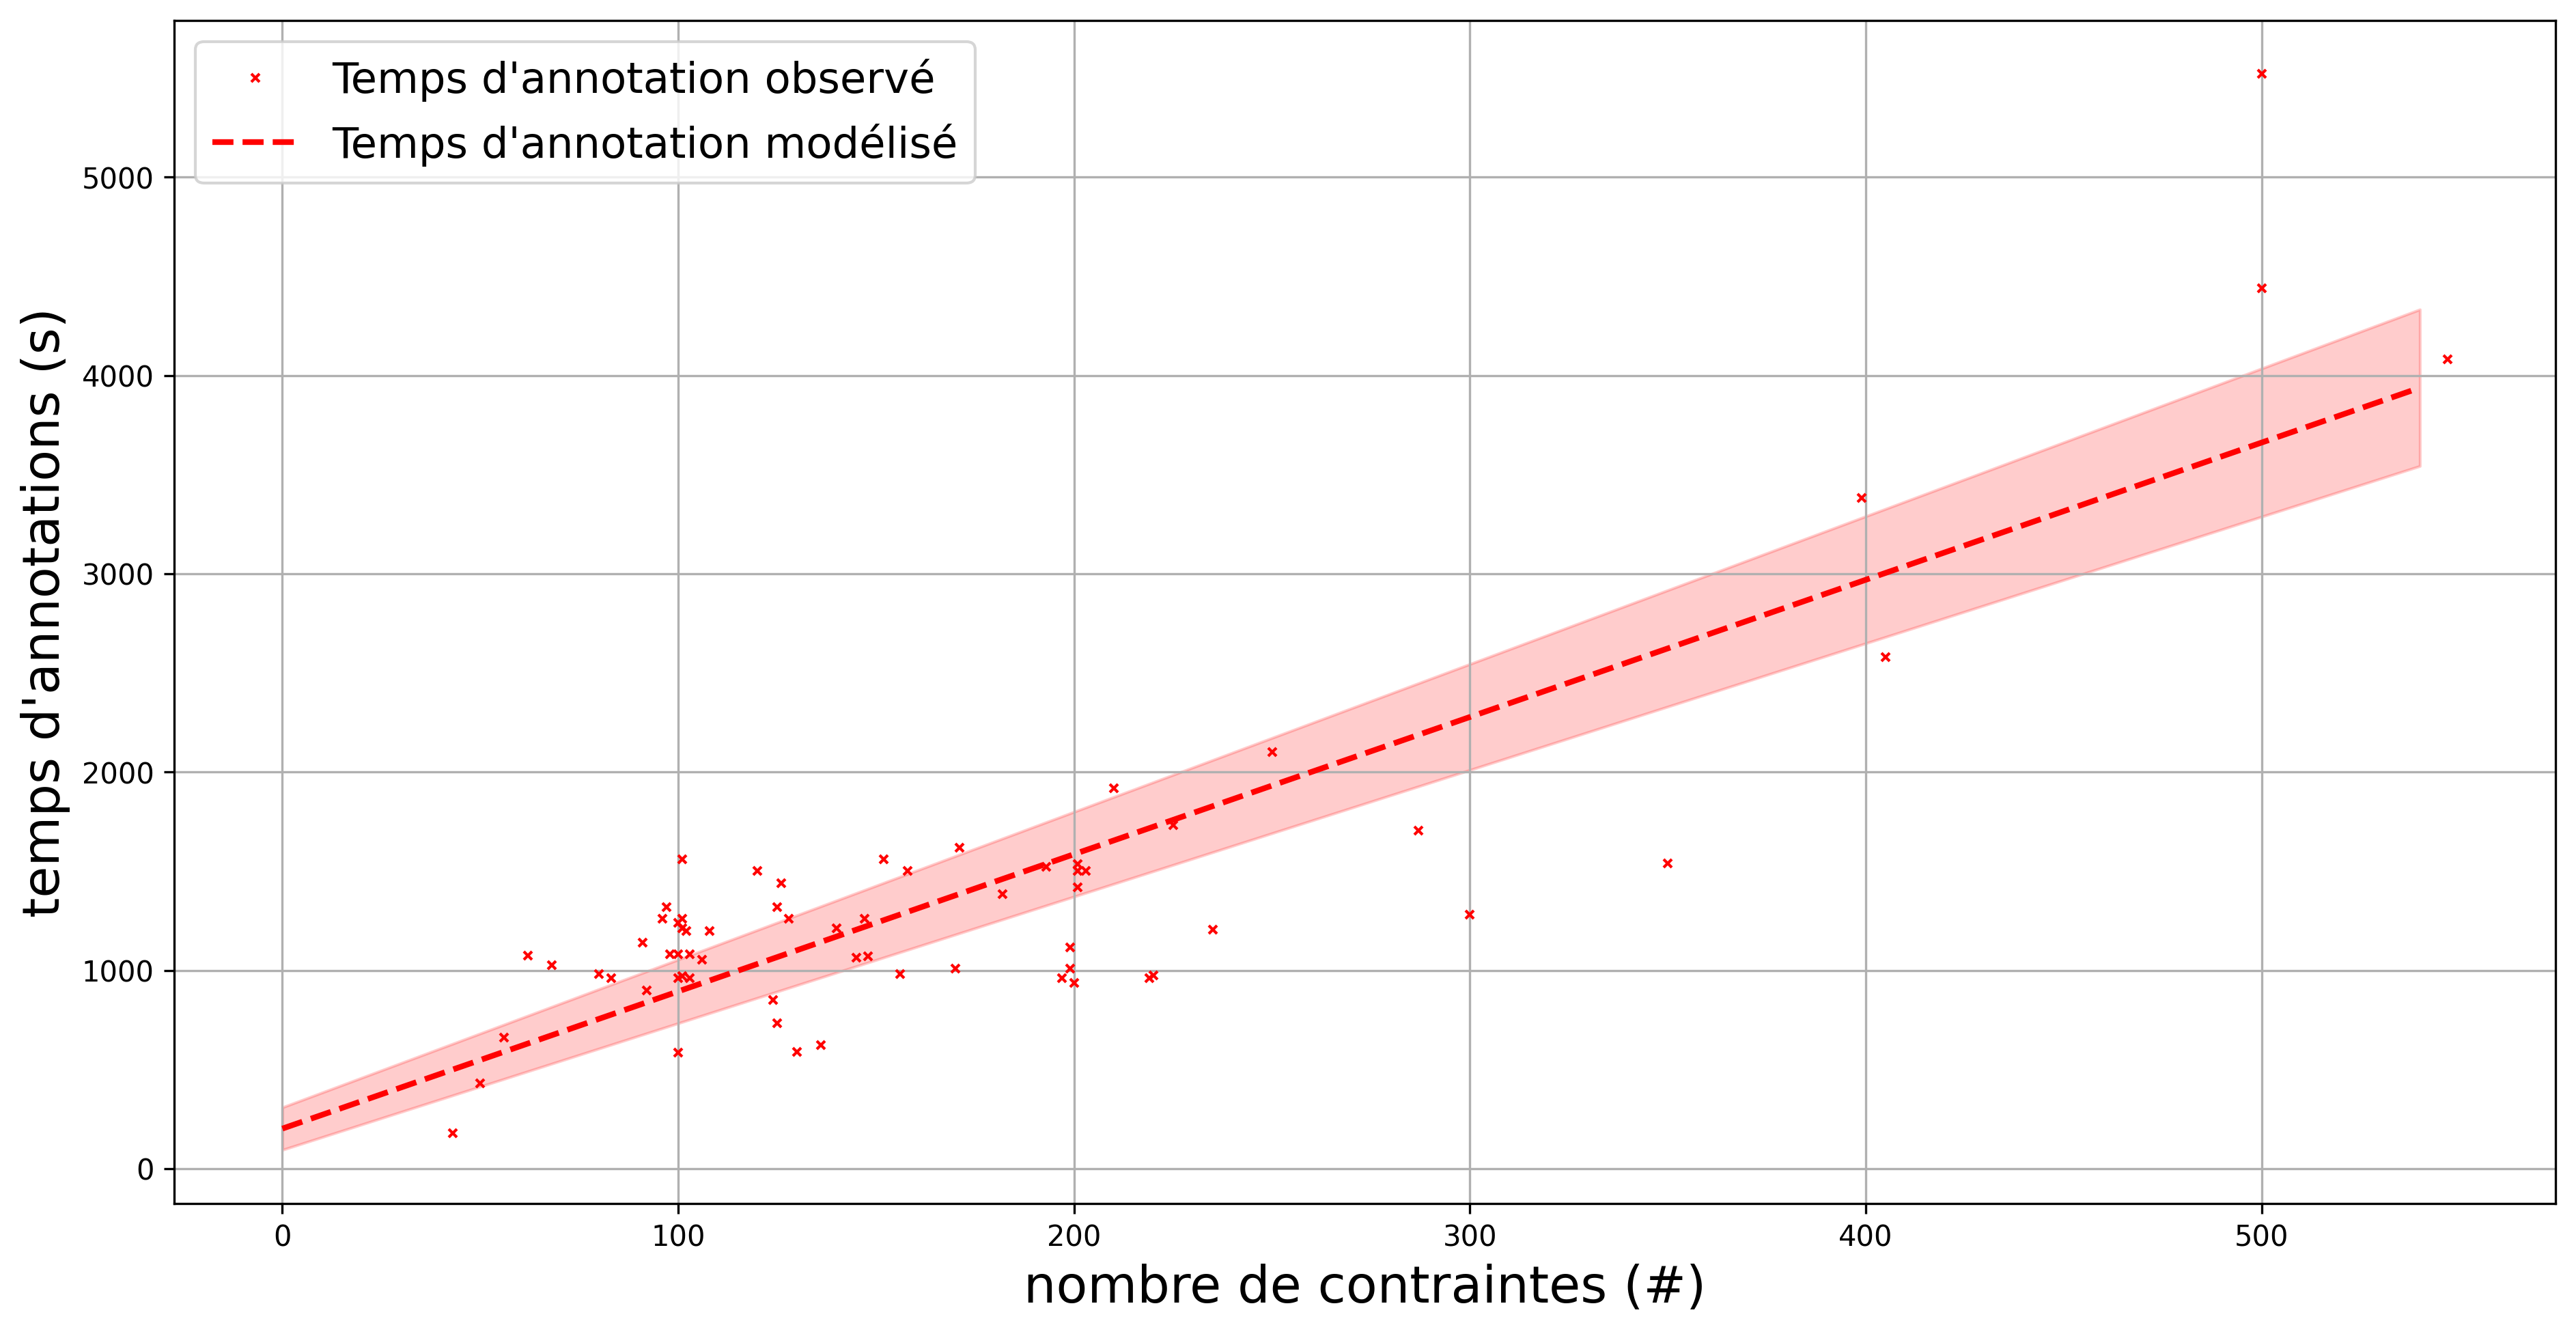
\includegraphics[width=\textwidth]{figures/etude-temps-annotation-1-modelisation-temps}
				\caption{Estimation du temps nécessaire (en secondes) pour annoter un lot de contraintes.}
				\label{figure:4.3.1-ETUDE-COUTS-TEMPS-ANNOTATION-SIMULATION}
			\end{figure}
		
			% Complément: Temps d'annotation d'une annotation partielle ou d'une annotation suffisante.
			\todo[inline]{RESULTATS TOTAUX POUR UNE ANNOTATION PARTIELLE / SUFFISANTE: Probablement mettre ces résultats dans la partie finale de cette section (pour 500 données : partielle=2.89heures, suffisante=5.27 heures)}
		%%	A l'aide de la modélisation temporelle réalisée ci-dessus, nous pouvons estimer qu'un lot de $50$ contraintes (comme employé dans nos précédentes études) nécessite en moyenne $548$ secondes, soit $9.13$ minutes.
		%%	De plus, en considérant les résultats de l'étude d'efficience (cf. section~\ref{section:4.2-HYPOTHESE-EFFICIENCE}) sur un jeu de $500$ points de données, nous pouvons déduire que :
		%%	\begin{itemize}
		%%		\item l'obtention d'une annotation partielle (atteindre $90$\% de \texttt{v-measure}) peut se faire avec $950$ contraintes, soit $19$ itérations de $50$ contraintes, ce qui équivaut à une moyenne de $2.89$ heures d'annotations ;
		%%		\item l'obtention d'une annotation suffisante (atteindre $100$\% de \texttt{v-measure}) peut se faire en $1~730$ contraintes, soit $34.6$ itérations de $50$ contraintes, ce qui équivaut à une moyenne de $5.27$ heures d'annotations.
		%%	\end{itemize}
		
			% Etude de cas.
			La figure~\ref{figure:4.3.1-ETUDE-COUTS-TEMPS-ANNOTATION-EXEMPLE} représente l'évolution de la vitesse d'annotation de quatre opérateurs (les deux plus rapides et les deux plus lents). Ces données sont l'objet d'une étude de cas dans la discussion ci-dessous.
			\todo{A SUPPRIMER car non essentiel ?}
			\begin{figure}[!htb]
				\centering
				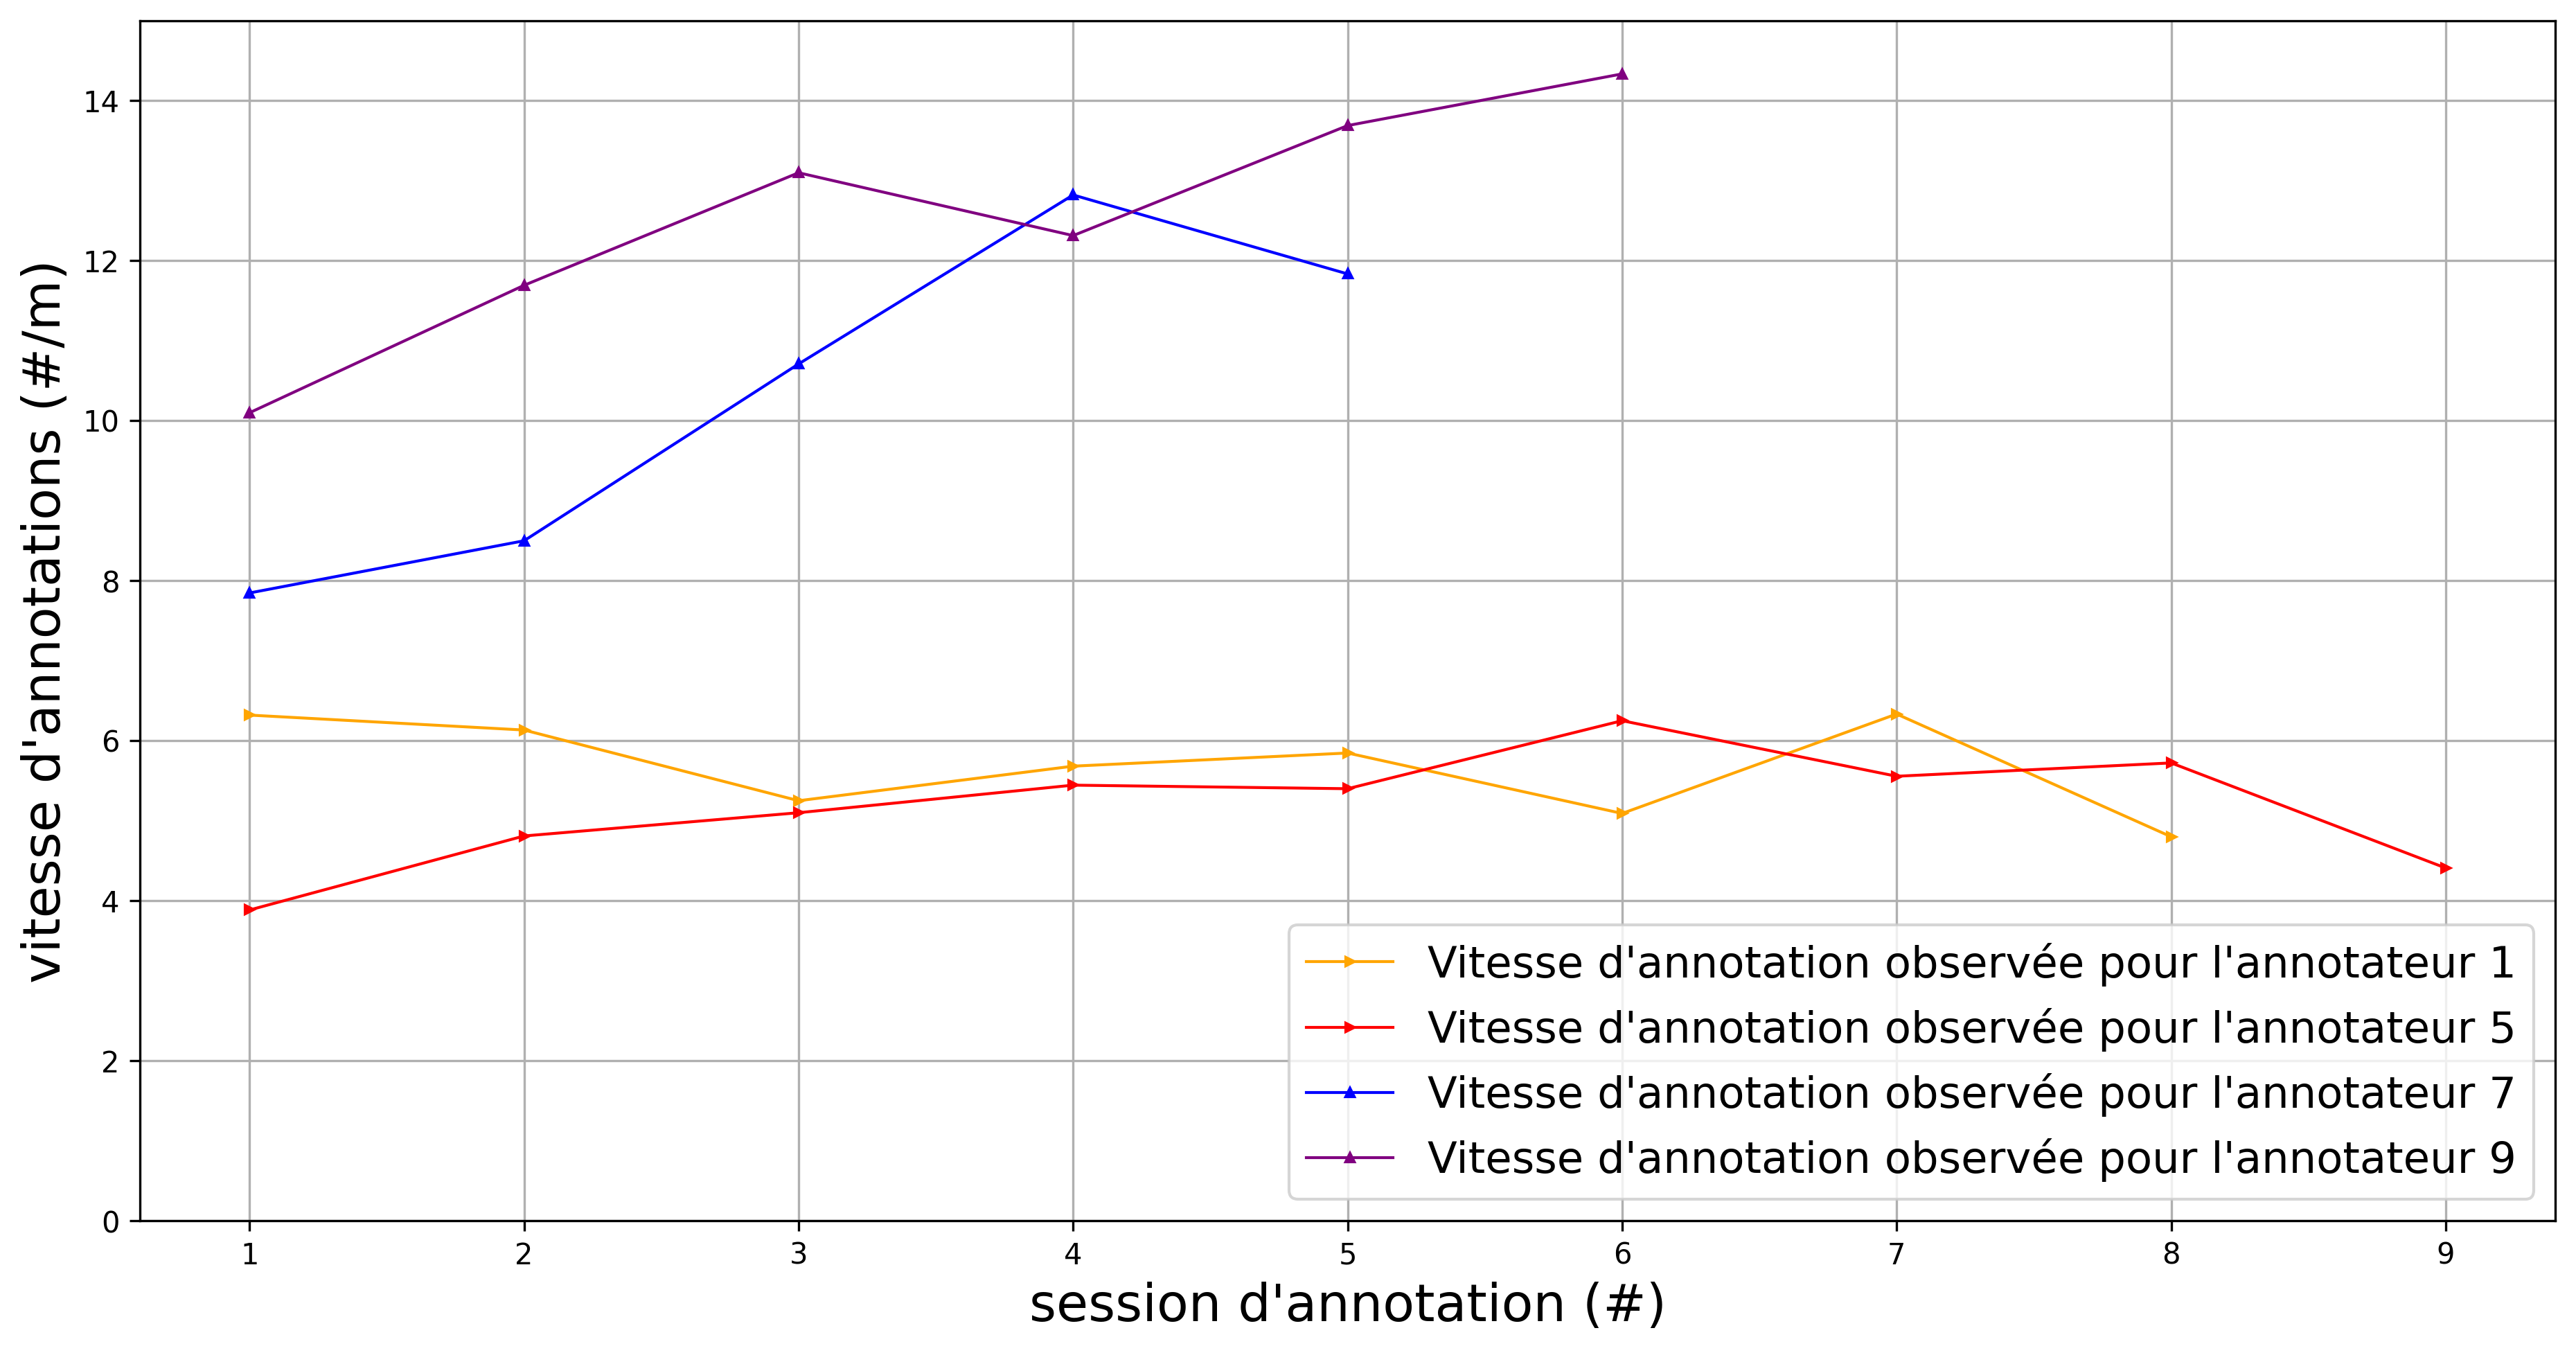
\includegraphics[width=\textwidth]{figures/etude-temps-annotation-3-etude-de-cas}
				\caption{Etude de cas d'évolution de la vitesse d'annotation de contraintes (en contraintes par minutes) en fonction des différentes sessions d'annotations}
				\label{figure:4.3.1-ETUDE-COUTS-TEMPS-ANNOTATION-EXEMPLE}
			\end{figure}

		%%% Discussion
		\subsubsection{Discussion}
		
		%%	\paragraph{Analyse du temps nécessaire :}
			% Généralités sur la modélisation du temps d'annotation sur une session.
			L'étude réalisée avec $14$ annotateurs sur des lots de $1~000$ contraintes a permis d'estimer à $202 + 6.92 \cdot \texttt{constraints\_number}$ le temps nécessaire (en secondes) pour annoter un lot de contraintes.
			Malgré une forte dispersion des résultats, cette modélisation permet de confirmer les tendances suivantes :
			\begin{itemize}
				\item Nous avons un \textbf{coût fixe} (environ $200$ secondes), qui peut représenter une partie du temps d'adaptation nécessaire à l'opérateur pour commencer sa tâche \todo{citation: Anderson (2013)} : cela comprend le temps de s'habituer à la tâche et de (ré)intégrer le contexte du sujet traité ;
				\item Nous avons un \textbf{coût variable faible} (inférieur à $7$ secondes par contrainte), qui concorde avec l'hypothèse d'une caractérisation rapide d'une similitude ou d'une différence entre deux données \todo{citation: Kahneman (2011), Hancock (1988)}.
			\end{itemize}
			Afin de \textbf{rentabiliser} le coût fixe à investir, il peut être judicieux de ne pas définir des lots d’annotation trop petits. 
			Comme le nombre médian de contraintes annotées durant les sessions d'annotation de cette expérience est de $138$ (moyenne à $170.70$), nous pouvons par exemple fixer la taille par défaut des lots à $100$ contraintes ($14.9$ minutes) ou $150$ contraintes ($20.7$ minutes).
			Attention toutefois à ne pas faire des lots trop conséquents (au delà de $200$), d'une part pour garder l'aspect itératif et interactif de la méthode, et d'autre part pour ne pas atteindre un pallier de \textbf{fatigue de} l'annotateur.\todo{citation: Jones et al. (2015), Elkosantini et Gien (2009)}
			
		%%	\paragraph{Comparaison à d'autres références :}
			% Comparaison du temps dtotal d'annotation en fin de section
			Nous discuterons de la durée totale d'un projet d'annotation avec notre méthode lors de la discussion finale de cette section.
			\todo[inline]{DISCUSSION RESULTATS TOTAUX POUR UNE ANNOTATION PARTIELLE / SUFFISANTE: Probablement mettre ces discussions dans la partie finale de cette section (pour 500 données : partielle=2.89heures, suffisante=5.27 heures ; comparer à 3 références équivalentes de et deux bornes extrême de Snow et al. (2008))}
		
			% Commentaire sur la difficulté de comparer les durées totales.
		%%	En ce qui concerne les durées totales pour annoter un jeu de $500$ points de données, estimées respectivement à $2.89$ et à $5.27$ heures suivant les seuils d'annotation, il est difficile de discuter de leur compétitivité à cause du manque de repères concrets.
		%%	En effet, les références dépendent de la tâche d'annotation, des données manipulées, du nombre de choix proposés à l'opérateur, de la complexité sémantique des données, des compétences des annotateurs, ...
		%%	\footnote{De plus, la plupart des études des tâches d'annotation en \textit{machine learning} se concentrent sur la cohérence inter-annotateurs plutôt que sur le temps nécessaire.}
		%%	Pour pallier ce problème, nous proposons de comparer nos estimations de temps d'annotations grâce aux pistes ci-dessous.
		%%	Ces repères sont approximatifs et assez disparates, mais ils nous permettront de discuter des ordres de grandeurs à manipuler.
			
			% Cas de taches de complexité similaire.
		%%	D'une part, comparons nos estimations à trois exemples de tâches ayant une \textbf{complexité similaire} à la vérité terrain que nous manipulons lors de cette expérience. Ces points de repères font appel à la catégorisation du thème traité par des textes courts.
			%
		%%	\begin{enumerate}
		%%		% Conception du JDD bank cards.
		%%		\item Pour concevoir le jeu de données~\todo{citation: bank cards} ($10$ classes équilibrées, $500$ points de données) servant de vérité terrain aux études d'efficacité et d'efficience, nous avons requis approximativement $5$ heures, dont $2.5$ d'annotation
		%%		\footnote{La conception de $bank cards$ a demandé $\sim 2$ heure de définition du périmètre (1 personne), $\sim 2$ heures de collecte et d'annotation des étiquettes des données (1 personne), et $\sim 1$ heure de revue de la cohérence des annotations (2 personne)} ;
		%%		% Conception du JDD MLSUM subset.
		%%		\item Pour adapter le jeu de données~\todo{citation: mlsum} en~\todo{citation: mlsum subset SCHILD} ($14$ classes retenues, $744$ points de données sélectionnées sur un échantillon de $1~050$) servant de base à notre étude du coût de l'annotation, nous avons requis approximativement $5$ heures, dont $2$ d'annotation binaire
		%%		\footnote{L'adaptation de $TODO:mlsum$ a demandé $\sim 1$ heure de collecte des catégories les plus communes (1 personne), $\sim 2$ heures d'annotation binaire de la pertinence des données (2 personnes) et $\sim 2$ heures de revue de la cohérence des annotations (2 personne)} ;
		%%		% Article Cheap and Fast — But is it Good? (Word Sense Disambiguation)
		%%		\item Selon~\todo{citation: Snow et al. (2008) / Yuret (2007)}, qui délègue à \texttt{Amazon Mechanical Turk} l'annotation de phrases pour catégoriser leur contexte parmi trois possibilités préformatés, il faut $8.59$ heures pour étiqueter $1~770$ données. En pondérant cette approximation pour un jeu de $500$ points de données, on peut estimer le temps d'annotation à $2.43$ heures environ ;
		%%	\end{enumerate}
			%
		%%	À l'aide de ces trois exemples, on remarque qu'une annotation partielle ($950$ contraintes pour atteindre $90$\% de \texttt{v-measure}) nécessite une durée comparable à une annotation par label ($2.89$ heures vs. entre $2$ et $3$ heures), mais une annotation suffisante ($1~730$ contraintes pour atteindre $100$\% de \texttt{v-measure}) nécessite 2 à 3 fois plus de temps ($5.27$ heures).
		%%	Il est donc préférable de nous concentrer sur une \textbf{annotation partielle} afin de garder une méthode efficiente. \todo{lien vers la section 4.4 a faire dans la discussion globale de cette section}
				% Ce choix implique de pouvoir compléter la différence qualité en remaniant manuellement certains \textit{clusters} obtenus lors d'une phase de revue.
				% Cet aspect sera complété à partir de l'étude décrite dans la section~\ref{section:4.4-HYPOTHESE-PERTINENCE} (hypothèse de pertinence).
			
			% cas de taches de complexité différentes
		%%	D'autre part, comparons nos estimations à deux exemples de tâches ayant des \textbf{complexité différentes} (une premier presque triviale, une seconde plutôt complexe) :
			%
		%%	\begin{enumerate}
		%%		\setcounter{enumi}{3}
		%%		% Article Cheap and Fast — But is it Good? (Word Similarity)
		%%		\item Selon~\todo{citation: Snow et al. (2008) / Rubenstein et Goodenough (1965)}, qui délègue à \texttt{Amazon Mechanical Turk} l'annotation de couples de mots pour identifier par similarité des synonymes, il faut $0.17$ heures pour ordonner $300$ paires de données de la plus à la moins similair
		%%		\footnote{La tâche d'annotation de synonymes par ordonnancement peut s'apparenter à de l'annotation de contraintes en se demandant : « \textit{laquelle de ces deux paires est la plus adéquate ? »}. Cette tâche est relativement simple (similarité intrinsèque triviale, peu de vocabulaire).}. En pondérant cette approximation pour un lot de $950$ contraintes, on peut estimer le temps d'annotation à environ $0.53$ heures ;
		%%		% Article Cheap and Fast — But is it Good? (Recognizing Textual Entailment)
		%%		\item Encore selon~\todo{citation: Snow et al. (2008) / Dagan et Magnini (2005)}, qui délègue à \texttt{Amazon Mechanical Turk} l'annotation binaire de la véracité d'une implication, il faut $89.3$ heures pour étiqueter $8~000$ données
		%%		\footnote{La tâche d'annotation de la véracité d'une implication peut s'apparenter à de l'annotation de contraintes en se demandant : « \textit{est-ce que l'implication est vraie ? »}. Cette tâche est relativement complexe (implication logique non trivial). }. En pondérant cette approximation pour un lot de $950$ contraintes, on peut estimer le temps d'annotation à environ $10.60$ heures ;
		%%	\end{enumerate}
			%
		%%	Avec ces deux exemples, on constate que les variations peuvent être très grandes (allant du cinquième au quadruple !).
		%%	Il est donc important de nuancer nos précédentes conclusions en fonction de la complexité de la thématique traitée.
		%%	Toutefois, 
		%%	\todo[inline]{données intrinsèquement différentes : peuvent être caractérisées très rapidement}
		%%	\todo[inline]{données ambiguës : peuvent demander plus de temps, plus de réflexion}
			
		%%	\paragraph{Autres études :}
			% Autres analyses sans conclusions
			Sur d'autres aspects, nous avons analysé l'évolution de la vitesse d'annotation au cours des sessions d'annotation, en espérant observer une accélération des annotations au fur et à mesure que l'annotateur s'habitue avec la tâche. Cependant, aucune de nos analyses n'a montré de résultats significatifs.
			Nous ne pouvons donc pas conclure sur de telles tendances.
			\begin{leftBarAuthorOpinion}
				Nos intuitions initiales concernaient trois points :
				\begin{itemize}
					\item la diminution du \textbf{temps d'adaptation} au cours de sessions d'annotations : au fur et à mesure qu'il annote, l'opérateur pourrait entrer plus facilement dans sa tâche, lui permettant d'atteindre plus rapidement sa vitesse de croisière et ainsi gagner en efficacité sur plusieurs sessions ;
					\item l'intervention d'\textbf{effet de fatigue} : si une session d'annotation dure trop longtemps, l'opérateur pourrait perdre en efficacité par manque de concentration et augmenter ses chances de faire des erreurs.
				\end{itemize}
				Ces différentes intuitions ont aussi été remontées par les annotateurs de notre expériences, mais aucun effet significatif n'a pu être observé.
				Cela est probablement dû au faible nombre d'opérateurs que nous avions à disposition pour cette expérience, à la forte disparité de ces individus (cf. figure\ref{figure:4.3.1-ETUDE-COUTS-TEMPS-ANNOTATION-EXEMPLE} où deux opérateurs sont constants alors que deux autres semblent s'améliorer au cours des sessions), ou encore à cause de leurs affinités avec l'application dont l'ergonomie doit jouer un rôle important.
			\end{leftBarAuthorOpinion}
			\todo{citation: Anderson (2013), Nielsen (1993)}
			\todo{citation: Jones et al. (2015), Elkosantini et Gien (2009)}
	

	%%%
	%%% Subsection 4.3.2: Étude du temps de calcul nécessaire aux algorithmes implémentés en chronométrant des exécutions dans différentes situations
	%%%
	\subsection{Étude du temps de calcul nécessaire aux algorithmes implémentés en chronométrant des exécutions dans différentes situations}
	\label{section:4.3.2-ETUDE-COUTS-TEMPS-CALCUL}
	
		%%% Protocole expérimental.
		\subsubsection{Protocole expérimental}
		
			% Transition.
			Maintenant que nous avons pu modéliser le temps nécessaire à un expert pour annoter un lot de contraintes, nous nous intéressons au temps nécessaire à la machine pour interpréter ces annotations et proposer une nouvelle segmentation des données.
			
			% Objectif de l'expérience.
			Pour cela, nous allons chronométrer plusieurs exécutions des algorithmes intervenant dans notre implémentation du \textit{clustering} interactif, et nous évaluerons l'importance de leurs différents arguments d'entrée (la taille du jeu de données, le nombre de clusters et le nombre de contraintes annotées, ...).
			Nous profiterons aussi de ces modélisations du temps de calcul pour confirmer le choix de paramétrage réalisé lors de l'étude d'efficience en section~\ref{section:4.2-HYPOTHESE-EFFICIENCE}, et ainsi faire un compromis entre l'algorithme le plus efficient et l'algorithme le plus rapide.
			
			% Remarques.
			\begin{leftBarWarning}
				Pour utiliser des jeux de données de tailles différentes tout en maîtrisant leur contenu, nous avons dupliqués aléatoirement des données issues de \textbf{TODO:JDD} en générant des fautes de frappes.
				Pour cette étude, nous faisons l'hypothèse que cela n'a pas d'impact majeur sur le temps d'exécution des différents algorithmes.
			\end{leftBarWarning}
			 \todo{TODO: reference dataset bank cards}
			
			% Pseudo-code.
			Pour résumer le protocole expérimental que nous décrivons ci-dessous, vous pouvez vous référer aux pseudo-code décrit dans Alg.~\ref{algorithm:4.3.2-ETUDE-COUTS-TEMPS-CALCUL-PROTOCOLE}.
			%
			\begin{algorithm}[!htb]
				\begin{algorithmic}[1]
					\Require jeux de données annotés (vérité terrain) de tailles différentes
					\ForAll{arrangement d'algorithmes et de paramètres à tester}
						\State \textbf{initialisation}: récupérer ou générer le jeu de données
						\If{estimation de la tâche de \textbf{prétraitement}}
							\State \textbf{chronomètre: START}
							\State \textbf{prétraitement (à étudier)}: supprimer le bruit dans les données
							\State \textbf{chronomètre: STOP}
						\ElsIf {estimation de la tâche de \textbf{vectorisation}}
							\State \textbf{prétraitement}: supprimer le bruit dans les données avec \texttt{prep.simple}
							\State \textbf{chronomètre: START}
							\State \textbf{vectorisation (à étudier)}: transformer les données en vecteurs
							\State \textbf{chronomètre: STOP}
						\ElsIf {estimation de la tâche de \textbf{clustering}}
							\State \textbf{prétraitement}: supprimer le bruit dans les données avec \texttt{prep.simple}
							\State \textbf{vectorisation}: transformer les données en vecteurs avec \texttt{vect.tfidf}
							\State \textbf{échantillonnage initial}: sélectionner une base de contraintes avec \texttt{samp.rand.full}
							\State \textbf{simulation d'annotation}: ajouter des contraintes en utilisant la vérité terrain
							\State \textbf{chronomètre: START}
							\State \textbf{clustering (à étudier)}: regrouper les données par similarité
							\State \textbf{chronomètre: STOP}
						\ElsIf {estimation de la tâche d'\textbf{échantillonnage}}
							\State \textbf{prétraitement}: supprimer le bruit dans les données avec \texttt{prep.simple}
							\State \textbf{vectorisation}: transformer les données en vecteurs avec \texttt{vect.tfidf}
							\State \textbf{échantillonnage initial}: sélectionner une base de contraintes avec \texttt{samp.rand.full}
							\State \textbf{simulation d'annotation}: ajouter des contraintes en utilisant la vérité terrain
							\State \textbf{clustering initial}: regrouper les données par similarité avec \texttt{clust.kmeans.cop}
							\State \textbf{chronomètre: START}
							\State \textbf{échantillonnage (à étudier)}: sélectionner de nouvelles contraintes à annoter
							\State \textbf{chronomètre: STOP}
						\EndIf
						\State \textbf{mesure}: estimer la différence de chronomètre pour cet algorithme
					\EndFor
					\ForAll{algorithme à modéliser}
						\State \textbf{cadrage}: définir les facteurs et les interactions intervenant dans la modélisation
						\State \textbf{simplification}: restreindre la modélisation aux facteurs les plus corrélés
						\State \textbf{modélisation}: entraîner un modèle linéaire généralisé avec les facteurs retenus
						\State \textbf{simulation}: écrire l'équation du temps d'exécution avec des paramètres obtenus
					\EndFor
					\Ensure modélisation du temps d'exécution des différents algorithmes
				\end{algorithmic}
				\caption{Description en pseudo-code du protocole expérimental de l'étude du temps d'exécution des algorithmes du \textit{clustering} interactif}
				\label{algorithm:4.3.2-ETUDE-COUTS-TEMPS-CALCUL-PROTOCOLE}
			\end{algorithm}
			
			% Description des tâches, des algorithmes et des contextes.
			Pour cette étude, nous lançons plusieurs exécutions de chaque algorithme de notre implémentation du \textit{clustering} interactif (cf. section~\ref{section:3.3-DESCRIPTION-IMPLEMENTATION}) avec différentes variations de contexte d'utilisation. Cela comprend les tâches, algorithmes et contextes d'utilisation suivants :
			%
			\begin{enumerate}
				% Prétraitement.
				\item le \textbf{prétraitement} des données...
					\begin{itemize}
						\item avec les algorithmes suivants : \textbf{simple} (noté \texttt{prep.simple}), \textbf{avec lemmatisation} (noté \texttt{prep.lemma}) et \textbf{avec filtres} (noté \texttt{prep.filter}) ;
						\item avec les contextes d'utilisation suivants : \textbf{nombre de données} (variant de $1~000$ à $5~000$ par pas de $1~000$, noté $\texttt{dataset\_size}$) ;
					\end{itemize}
				% Vectorisation.
				\item la \textbf{vectorisation} des données...
					\begin{itemize}
						\item avec les algorithmes suivants : \textbf{TF-IDF} (noté \texttt{vect.tfidf}) et \textbf{SpaCy} (noté \texttt{vect.frcorenewsmd}) ;
						\item avec les contextes d'utilisation suivants : \textbf{nombre de données} (variant de $1~000$ à $5~000$ par pas de $1~000$, noté $\texttt{dataset\_size}$) ;
						\item précédé par un prétraitement \textbf{simple} ;
					\end{itemize}
				% Clustering.
				\item le \textbf{\textit{clustering} sous contraintes} des données...
					\begin{itemize}
						\item avec les algorithmes suivants : \textbf{KMeans} (modèle \textit{COP} noté \texttt{clust.kmeans.cop}), \textbf{Hiérarchique} (lien \textit{single} noté \texttt{clust.hier.sing} ; lien \textit{complete} noté \texttt{clust.hier.comp} ; lien \textit{average} noté \texttt{clust.hier.avg} ; lien \textit{ward} noté \texttt{clust.hier.ward}) et \textbf{Spectral} (modèle \textit{SPEC} noté \texttt{clust.spec}) ;
						\item avec les contextes d'utilisation suivants : \textbf{nombre de données} (variant de $1~000$ à $5~000$ par pas de $1~000$, noté $\texttt{dataset\_size}$), le \textbf{nombre de contraintes annotés} (variant de $0$ à $5~000$ par pas de $500$, noté $\texttt{previous\_nb\_constraints}$) et le \textbf{nombre de \textit{clusters} à trouver} (variant de $5$ à $50$ par pas de $5$, noté $\texttt{algorithm\_nb\_clusters}$) ;
						\item précédé par un prétraitement \textbf{simple} et une vectorisation \textbf{TF-IDF} et un échantillonnage initial \textbf{purement aléatoire} ;
					\end{itemize}
				% Sampling.
				\item l'\textbf{échantillonnage} des contraintes à annoter...
					\begin{itemize}
						\item avec les algorithmes suivants : \textbf{purement aléatoire} (noté \texttt{samp.random.full}), \textbf{pseudo-aléatoire} (noté \texttt{samp.random.same}), \textbf{même cluster et étant les plus éloignées} (noté \texttt{samp.farhtest.same}) et \textbf{clusters différents et étant les plus proches} (noté \texttt{samp.closest.diff}) ;
						\item avec les contextes d'utilisation suivants : \textbf{nombre de données} (variant de $1~000$ à $5~000$ par pas de $1~000$, noté $\texttt{dataset\_size}$), le \textbf{nombre de contraintes annotés} (variant de $0$ à $5~000$ par pas de $500$, noté $\texttt{previous\_nb\_constraints}$), le \textbf{nombre de \textit{clusters} existant} (variant de $10$ à $50$ par pas de $10$, noté $\texttt{previous\_nb\_clusters}$) et le \textbf{nombre de contraintes à sélectionner} (variant de $50$ à $250$ par pas de $50$, noté $\texttt{algorithm\_nb\_constraints}$) ;
						\item précédé par un prétraitement \textbf{simple}, une vectorisation \textbf{TF-IDF}, un \textit{clustering} initial \textbf{KMeans} (modèle \textit{COP}) et un échantillonnage initial \textbf{purement aléatoire} ;
					\end{itemize}
			\end{enumerate}
			
			Il y a donc $8~825$ combinaisons d'algorithmes (\texttt{15} pour le prétraitement, $10$ pour la vectorisation, $3~330$ pour le \textit{clustering}, $5~550$ pour l'échantillonnage), et chaque combinaison est répétée $5$ fois pour contrer les aléas statistiques des exécutions.
			De plus, chaque jeu de données est généré $5$ fois pour contrer les aléas statistiques de création, donc il y a $220~625$ exécutions d'algorithmes ($375$ pour le prétraitement, $250$ pour la vectorisation, $82~500$ pour le \textit{clustering}, $137~500$ pour l'échantillonnage).
			
			% Description de la modélisation.
			Sur la base de ces mesures, nous cherchons à modéliser le temps d'exécution de chaque algorithme en fonction de son contexte d'utilisation (dépendant de ses arguments d'entrée), et les interactions doubles entre paramètres sont envisagées.
			Afin de réduire la complexité des modélisations, nous ordonnons les interactions de facteurs possibles en fonction de leur corrélation avec le temps mesuré (la corrélation \texttt{r} de \textit{Pearson} est utilisée) et nous nous limitons aux variables responsables d'un maximum de la variance des mesures (la méthode d'\textit{Elbow} est utilisée pour choisir les facteurs pertinents).
			Sur cette base, nous entraînons un modèle linéaire généralisé (\textit{GLM}) pour représenter le temps d'exécution moyen de l'algorithme : ce modèle sera caractérisé par le coefficient de détermination généralisé \texttt{R²} de \textit{Cox et Snel}, la log-vraisemblance \texttt{llf} et la log-vraisemblance \texttt{llf\_null} du modèle \textit{null}.
			Pour finir, nous discuterons des valeurs des coefficients obtenus sur l'impact du temps d'exécution.
			
			% Référence scripts.
			\begin{leftBarInformation}
				Ces analyses sont réalisées en Python à l'aide des librairies \texttt{datetime} et \texttt{statsmodels} (\cite{seabold:2010}).
				Les scripts de l'expérience (\textit{notebooks} Python) sont disponibles dans un dossier dédié de~\cite{schild:cognitivefactory-interactive-clustering-comparative-study:2021}.
			\end{leftBarInformation}

		%%% Résultats
		\subsubsection{Résultats obtenus}
				
			%%% Prétraitements
			
			% Première analyse.
			En ce qui concerne la tâche de \textbf{prétraitement}, une première analyse montre que les modélisations des trois implémentations sont similaires (\texttt{p-valeur}: $> 0.980$). Nous ferons donc une seule modélisation.
			
			% Modélisation du temps de calcul (prep.simple + prep.lemma + prep.filter).
			Pour les algorithmes de prétraitements (\texttt{prep.simple}, \texttt{prep.lemma} et \texttt{prep.filter}), l'analyse de la corrélation des facteurs avec les mesures de temps d'exécution indique qu'une modélisation minimale et suffisante peut être réalisée à partir du facteur $\texttt{dataset\_size}$ (\texttt{r}: $0.997$).
			Le modèle linéaire généralisé retenu (\texttt{R²}: $> 0.999$, \texttt{llf}: $-379.35$, \texttt{llf\_null}: $-1~353.98$) nous permet de déduire l'équation suivante\todo{ref complexité théorique algo en annexe} :
			%
			\begin{equation}
				time.prep~(secondes)~
				\simeq~0.84 + 6.31 \cdot 10^{-3} \cdot \texttt{dataset\_size}
			\end{equation}
			
			% Affichage du temps de calcul.
			La figure~\ref{figure:4.3.2-ETUDE-COUTS-TEMPS-CALCUL-MODELISATION-PREPROCESSING} représente cette modélisation du temps de calcul des algorithmes de prétraitements en comparaison avec les mesures réalisées lors de l'expérience.
			\newline
			%		
			\begin{figure}[!htb]
				\centering
				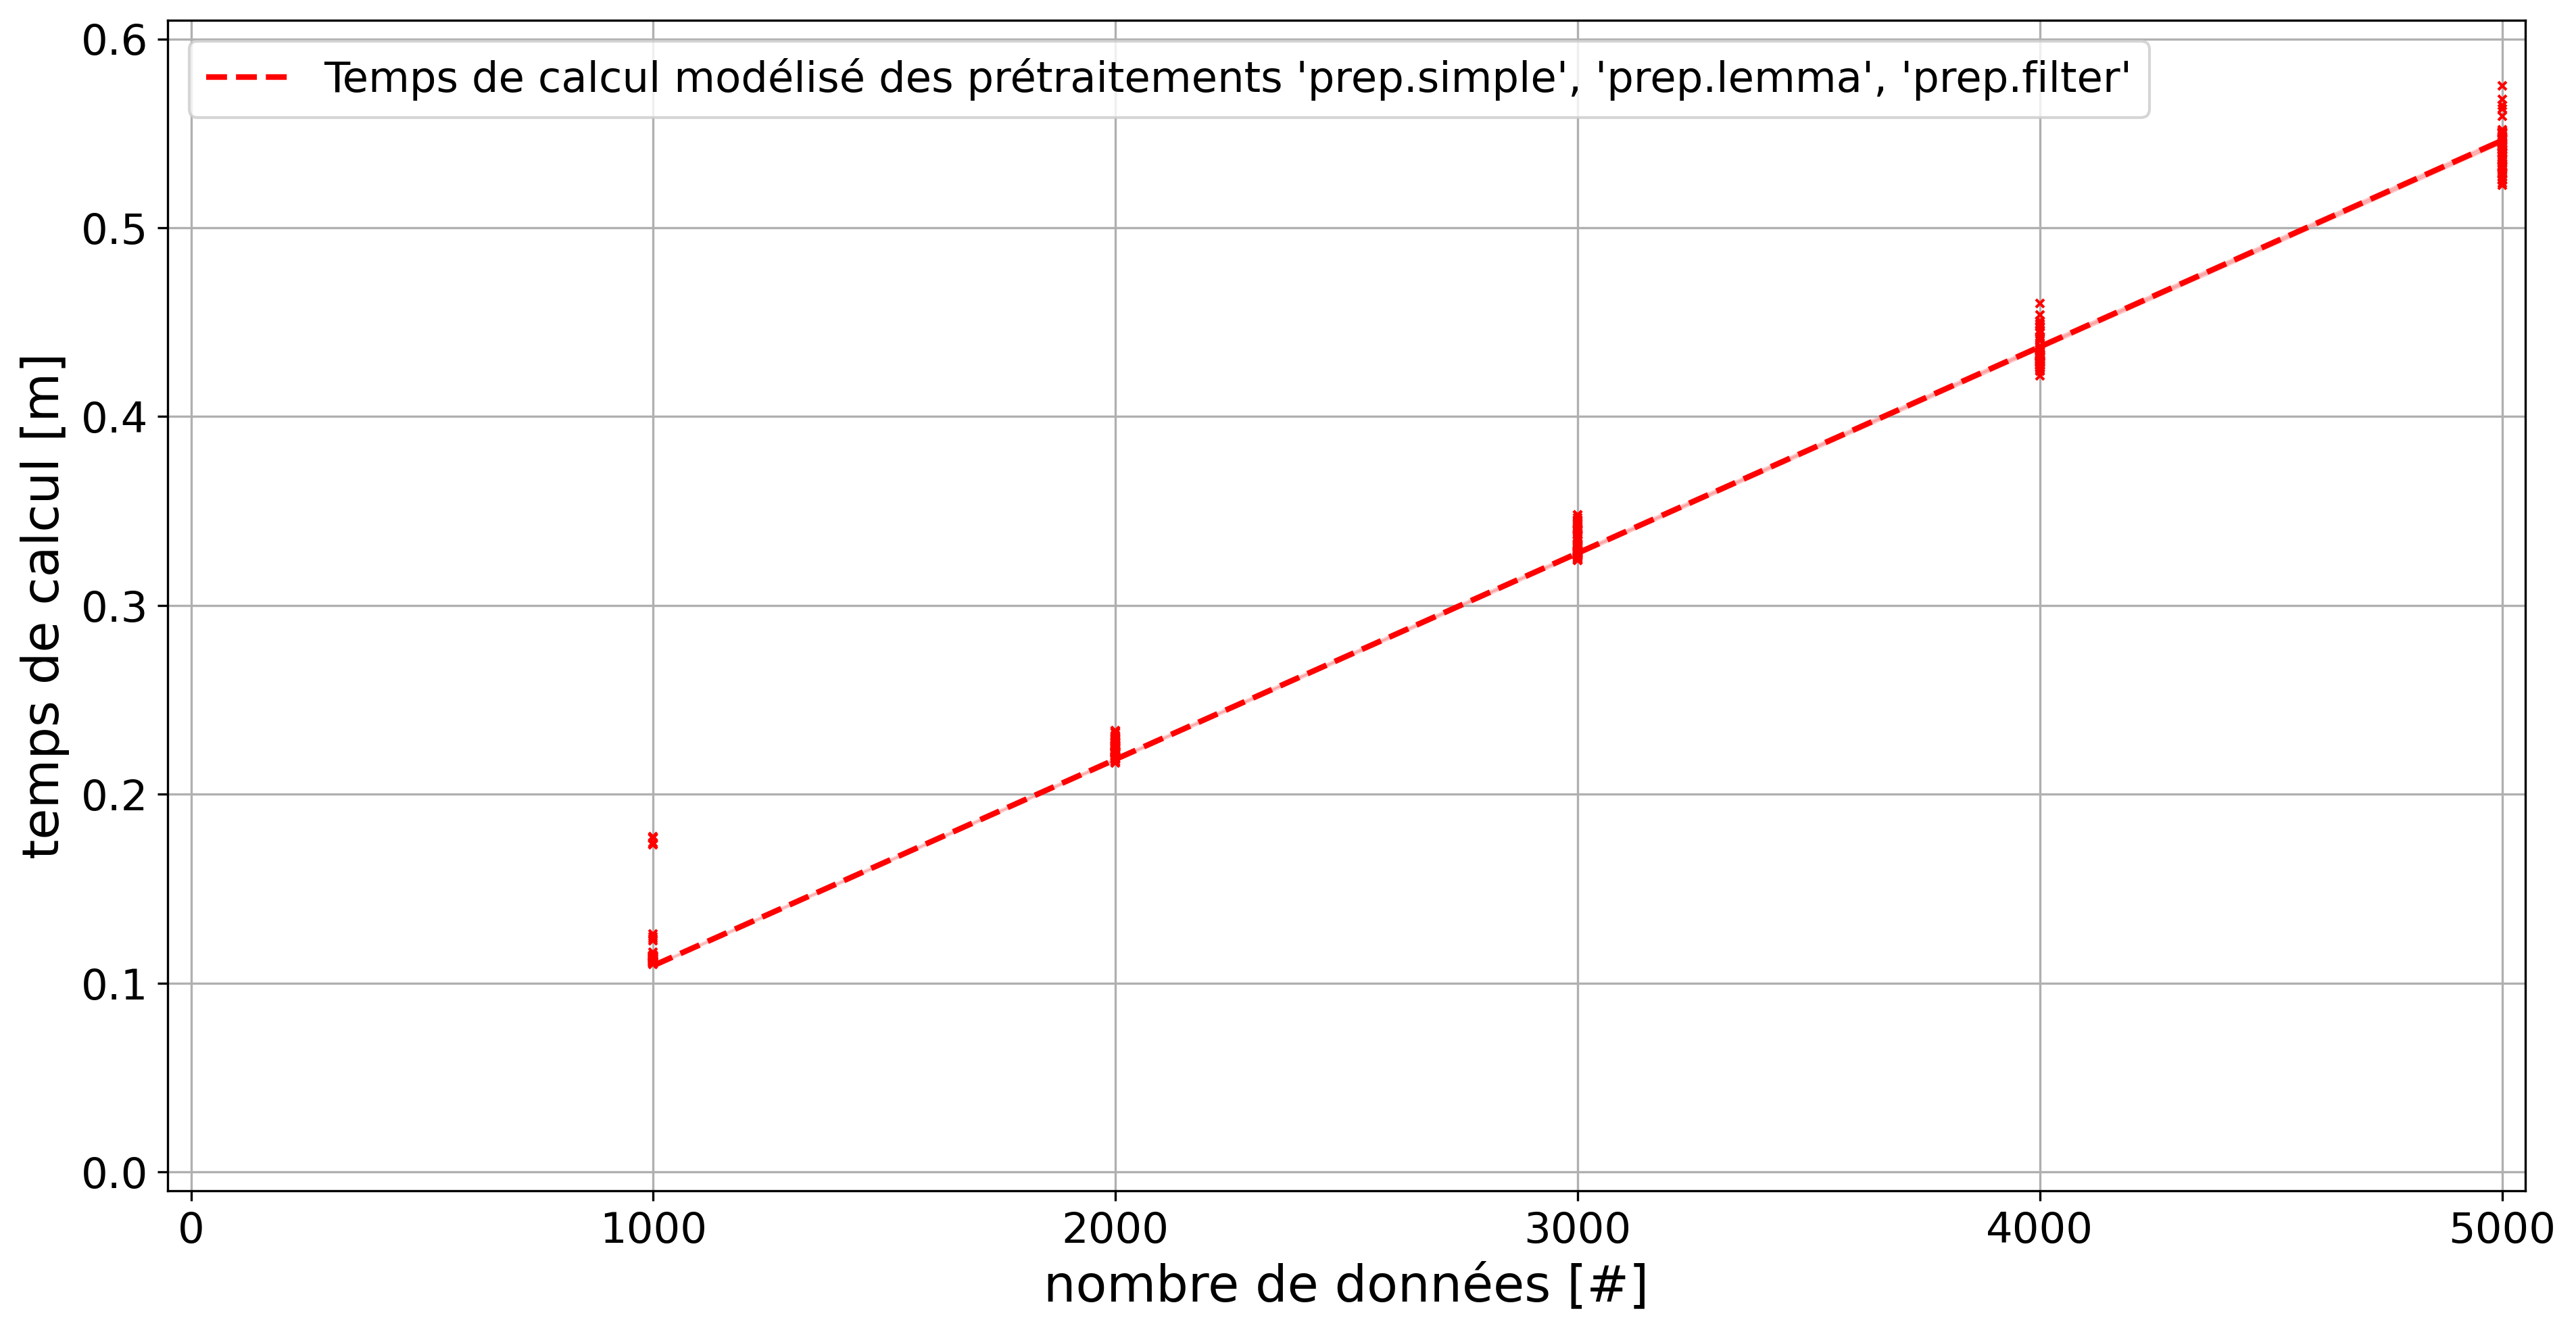
\includegraphics[width=0.8\textwidth]{figures/etude-temps-calcul-modelisation-1prep}
				\caption{Estimation du temps nécessaire (en secondes) pour effectuer une tâche de \textbf{prétraitement} en fonction du nombre de données à traiter. Les paramétrages \texttt{prep.simple}, \texttt{prep.lemma} et \texttt{prep.filter} ayant des temps de calculs similaires, leurs modélisations n'ont pas été séparées.}
				\label{figure:4.3.2-ETUDE-COUTS-TEMPS-CALCUL-MODELISATION-PREPROCESSING}
			\end{figure}
			
			%%% Vectorization
			
			% Première analyse.
			En ce qui concerne la tâche de \textbf{vectorisation}, une première analyse montre que les modélisations des deux implémentations sont différentiables  (\texttt{p-valeur}: $< 10^{-3}$). Nous ferons donc une modélisation par algorithme.
		
			% Modélisation du temps de calcul (vect.tfidf).
			Pour les algorithmes de vectorisation \texttt{vect.tfidf}, l'analyse de la corrélation des facteurs avec les mesures de temps d'exécution indique qu'une modélisation minimale et suffisante peut être réalisée à partir du facteur $\texttt{dataset\_size}$ (\texttt{r}: $0.977$).
			Le modèle linéaire généralisé retenu (\texttt{R²}: $> 0.999$, \texttt{llf}: $262.35$, \texttt{llf\_null}: $70.04$) nous permet de déduire l'équation suivante\todo{ref complexité théorique algo en annexe} :
			%
			\begin{equation}
				time.vect.tfidf~(secondes)~
				\simeq~-0.014 + 9.54 \cdot 10^{-5} \cdot \texttt{dataset\_size}
			\end{equation}
			
			% Modélisation du temps de calcul (vect.frcorenewsmd).
			Pour les algorithmes de vectorisation \texttt{vect.frcorenewsmd}, l'analyse de la corrélation des facteurs avec les mesures de temps d'exécution indique qu'une modélisation minimale et suffisante peut être réalisée à partir du facteur $\texttt{dataset\_size}$ (\texttt{r}: $0.983$).
			Le modèle linéaire généralisé retenu (\texttt{R²}: $> 0.999$, \texttt{llf}: $-186.80$, \texttt{llf\_null}: $-399.39$) nous permet de déduire l'équation suivante\todo{ref complexité théorique algo en annexe} :
			%
			\begin{equation}
				time.vect.frcorenewsmd~(secondes)~
				\simeq~1.89 + 4.11 \cdot 10^{-3} \cdot \texttt{dataset\_size}
			\end{equation}
			
			% Affichage du temps de calcul.
			La figure~\ref{figure:4.3.2-ETUDE-COUTS-TEMPS-CALCUL-MODELISATION-VECTORIZATION} représente ces modélisations de temps de calcul des algorithmes de vectorisation en comparaison avec les mesures réalisées lors de l'expérience.
			\newline
			%
			\begin{figure}[!htb]
				\centering
				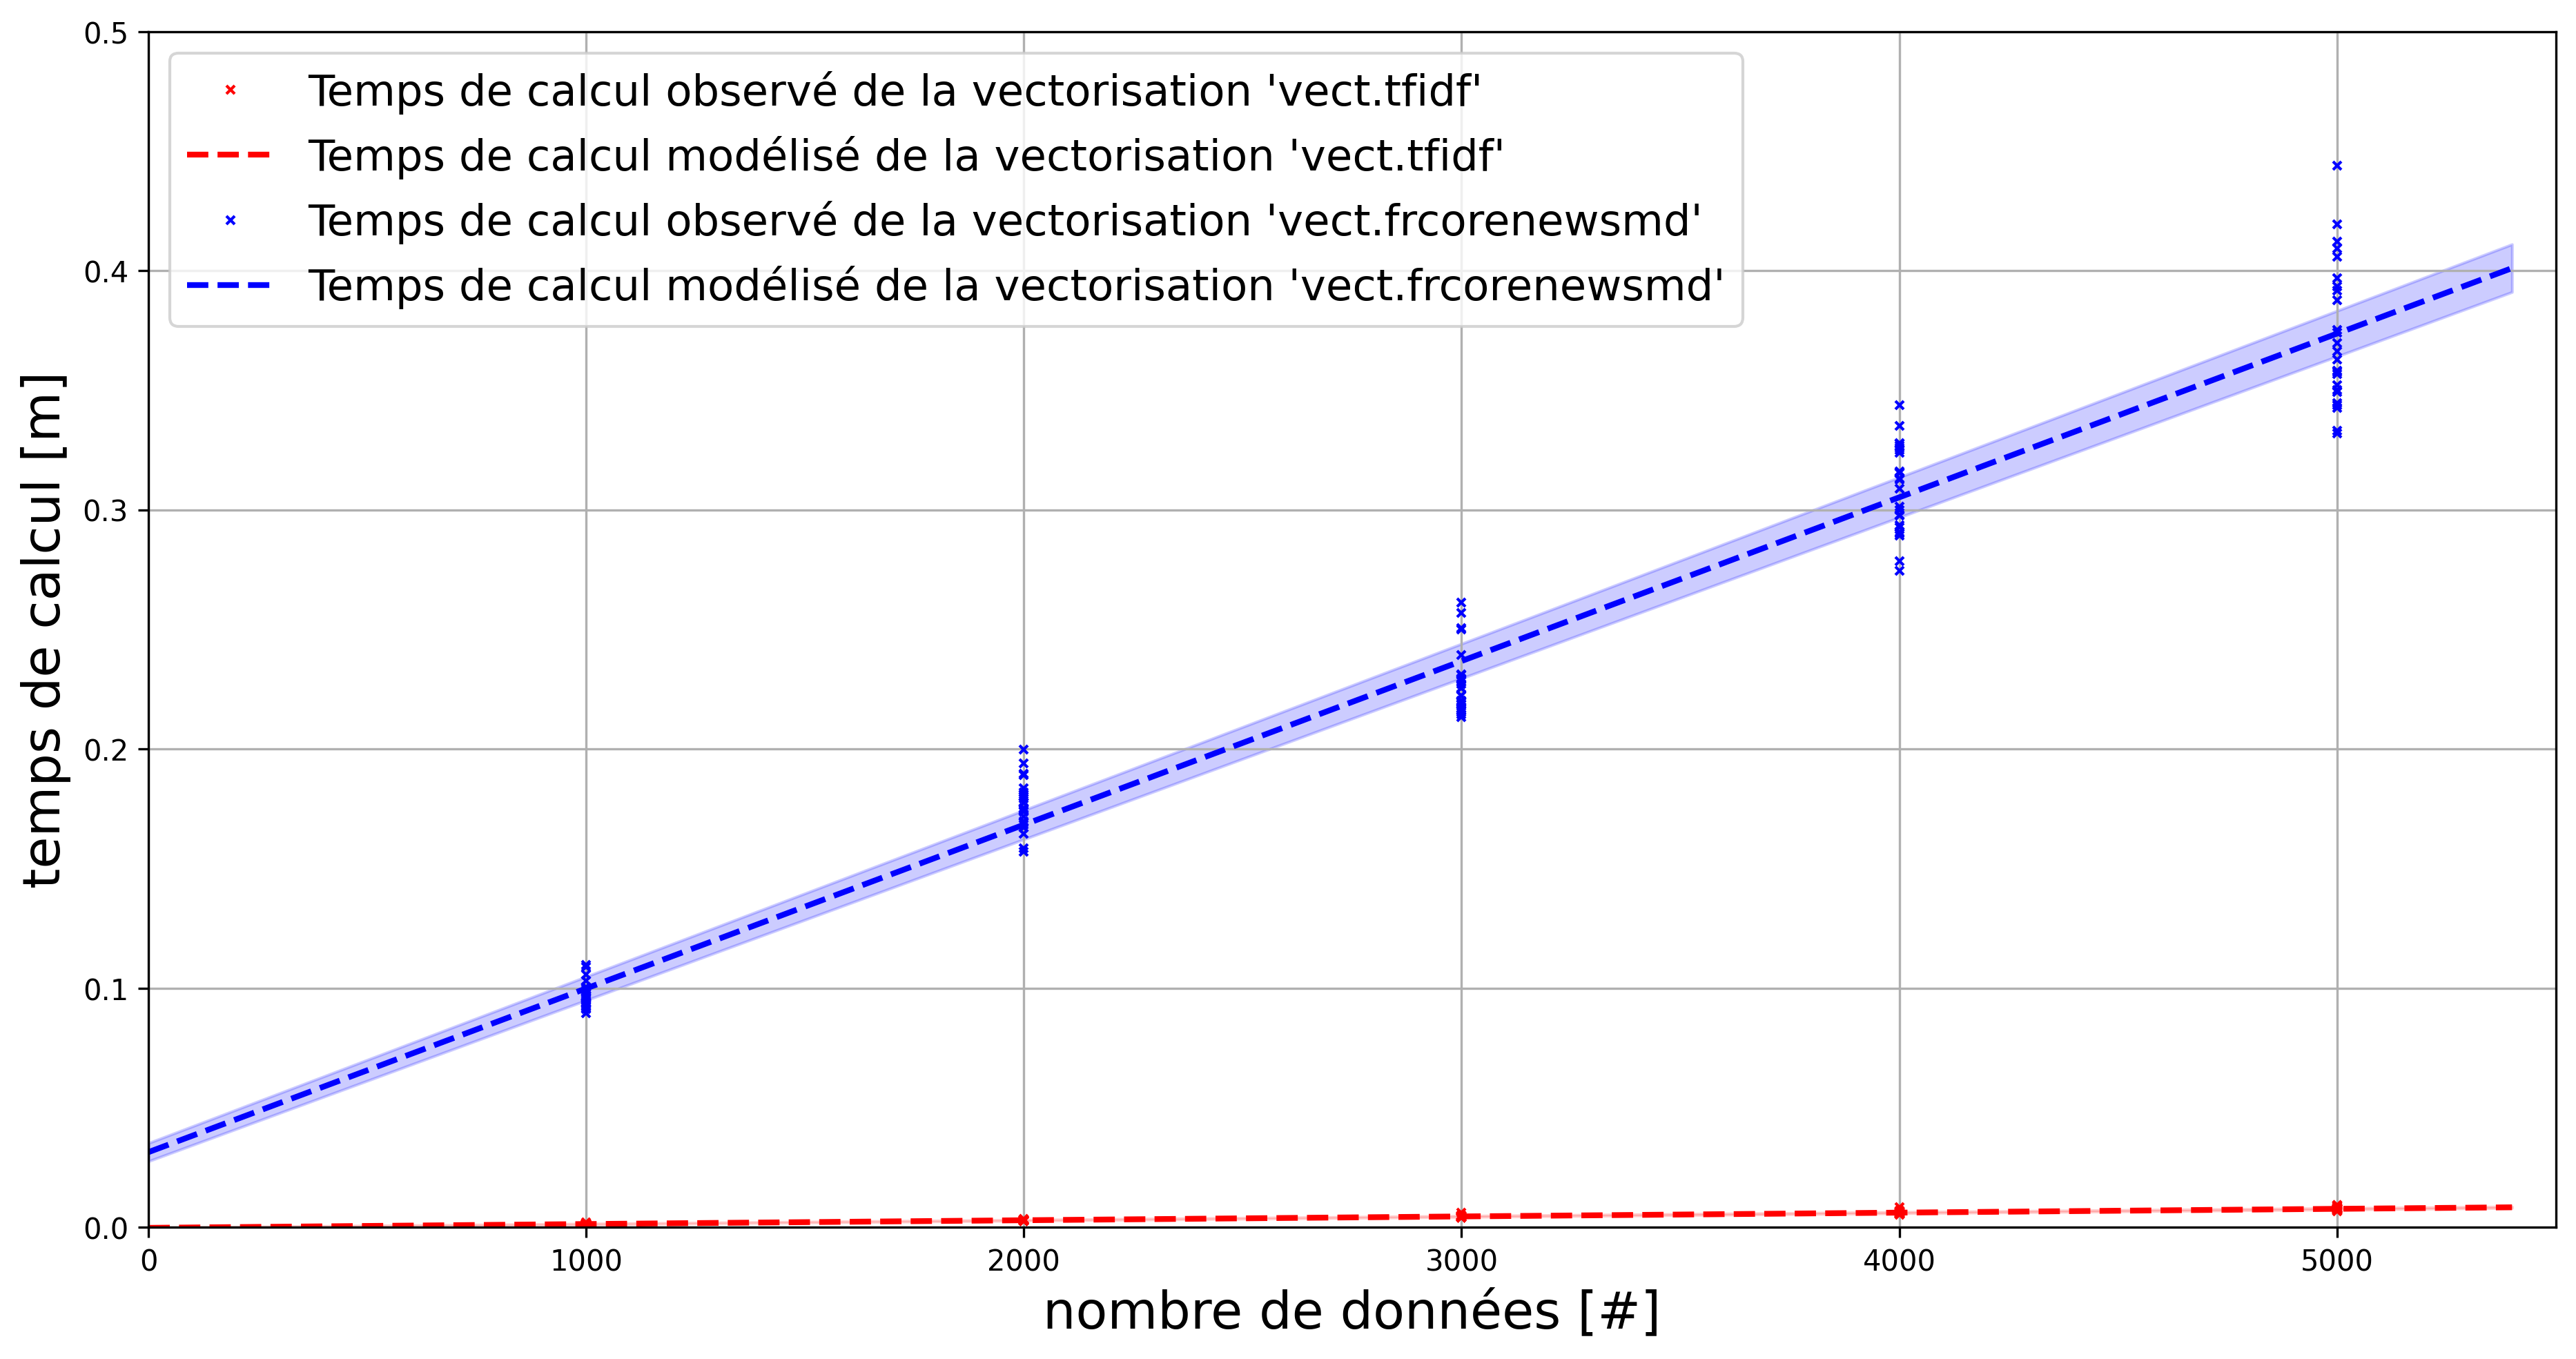
\includegraphics[width=0.8\textwidth]{figures/etude-temps-calcul-modelisation-2vect}
				\caption{Estimation du temps nécessaire (en secondes) pour effectuer une tâche de \textbf{vectorisation} en fonction du nombre de données à traiter.}
				\label{figure:4.3.2-ETUDE-COUTS-TEMPS-CALCUL-MODELISATION-VECTORIZATION}
			\end{figure}
			
			%%% Clustering
			
			% Première analyse.
			En ce qui concerne la tâche de \textbf{\textit{clustering} sous contraintes}, une première analyse montre que les modélisations des six implémentations sont différentiables  (\texttt{p-valeur}: $<$ \texttt{$10^{-3}$}). Nous ferons donc une modélisation par algorithme.
			
			% Modélisation du temps de calcul (clust.kmeans.cop).
			Pour les algorithmes du \textit{clustering} sous contraintes \texttt{clust.kmeans.cop}, l'analyse de la corrélation des facteurs avec les mesures de temps d'exécution indique qu'une modélisation minimale et suffisante peut être réalisée à partir du facteur $\texttt{dataset\_size}$ (\texttt{r}: $0.837$).
			Le second facteur le plus corrélé (mais non retenu) est l'interaction $\texttt{dataset\_size}^{2} \cdot algorithm\_nb\_clusters$ (\texttt{r}: $0.545$).
			Le modèle linéaire généralisé retenu (\texttt{R²}: $0.904$, \texttt{llf}: $-9.20 \cdot 10^{4}$, \texttt{llf\_null}: $-1.00 \cdot 10^{5}$) nous permet de déduire l'équation suivante\todo{ref complexité théorique algo en annexe} :
			%
			\begin{equation}
				time.clust.kmeans.cop~(secondes)~
				\simeq~-240 + 2.11 \cdot 10^{-1} \cdot \texttt{dataset\_size}
			\end{equation}
			
			% Modélisation du temps de calcul (clust.hier.sing).
			Pour les algorithmes du \textit{clustering} sous contraintes \texttt{clust.hier.sing}, l'analyse de la corrélation des facteurs avec les mesures de temps d'exécution indique qu'une modélisation minimale et suffisante peut être réalisée à partir du facteur $\texttt{dataset\_size}^{2}$ (\texttt{r}: $0.940$).
			Le second facteur le plus corrélé (mais non retenu) est l'interaction $\texttt{dataset\_size}^{2} \cdot algorithm\_nb\_clusters$ (\texttt{r}: $0.729$).
			Le modèle linéaire généralisé retenu (\texttt{R²}: $> 0.999$, \texttt{llf}: $-5.38 \cdot 10^{4}$, \texttt{llf\_null}: $-6.10 \cdot 10^{4}$) nous permet de déduire l'équation suivante\todo{ref complexité théorique algo en annexe} :
			%
			\begin{equation}
				time.clust.hier.sing~(secondes)~
				\simeq~-887 + 6.37 \cdot 10^{-4} \cdot \texttt{dataset\_size}^{2}
			\end{equation}
			
			% Modélisation du temps de calcul (clust.hier.comp).
			Pour les algorithmes du \textit{clustering} sous contraintes \texttt{clust.hier.comp}, l'analyse de la corrélation des facteurs avec les mesures de temps d'exécution indique qu'une modélisation minimale et suffisante peut être réalisée à partir du facteur $\texttt{dataset\_size}^{2}$ (\texttt{r}: $0.938$).
			Le second facteur le plus corrélé (mais non retenu) est l'interaction $\texttt{dataset\_size}^{2} \cdot algorithm\_nb\_clusters$ (\texttt{r}: $0.736$).
			Le modèle linéaire généralisé retenu (\texttt{R²}: $> 0.999$, \texttt{llf}: $-5.40 \cdot 10^{4}$, \texttt{llf\_null}: $-6.11 \cdot 10^{4}$) nous permet de déduire l'équation suivante\todo{ref complexité théorique algo en annexe} :
			%
			\begin{equation}
				time.clust.hier.comp~(secondes)~
				\simeq~-925 + 6.42 \cdot 10^{-4} \cdot \texttt{dataset\_size}^{2}
			\end{equation}

			% Modélisation du temps de calcul (clust.hier.avg).
			Pour les algorithmes du \textit{clustering} sous contraintes \texttt{clust.hier.avg}, l'analyse de la corrélation des facteurs avec les mesures de temps d'exécution indique qu'une modélisation minimale et suffisante peut être réalisée à partir du facteur $\texttt{dataset\_size}^{2}$ (\texttt{r}: $0.915$).
			Le second facteur le plus corrélé (mais non retenu) est l'interaction $\texttt{dataset\_size}^{2} \cdot algorithm\_nb\_clusters$ (\texttt{r}: $0.713$).
			Le modèle linéaire généralisé retenu (\texttt{R²}: $0.942$, \texttt{llf}: $-5.82 \cdot 10^{4}$, \texttt{llf\_null}: $-6.45 \cdot 10^{4}$) nous permet de déduire l'équation suivante\todo{ref complexité théorique algo en annexe} :
			%
			\begin{equation}
				time.clust.hier.avg~(secondes)~
				\simeq~-1100 + 1.02 \cdot 10^{-3} \cdot \texttt{dataset\_size}^{2}
			\end{equation}

			% Modélisation du temps de calcul (clust.hier.ward).
			Pour les algorithmes du \textit{clustering} sous contraintes \texttt{clust.hier.ward}, l'analyse de la corrélation des facteurs avec les mesures de temps d'exécution indique qu'une modélisation minimale et suffisante peut être réalisée à partir du facteur $\texttt{dataset\_size}^{2}$ (\texttt{r}: $0.945$).
			Le second facteur le plus corrélé (mais non retenu) est l'interaction $\texttt{dataset\_size}^{2} \cdot algorithm\_nb\_clusters$ (\texttt{r}: $0.734$).
			Le modèle linéaire généralisé retenu (\texttt{R²}: $> 0.999$, \texttt{llf}: $-5.39 \cdot 10^{4}$, \texttt{llf\_null}: $-6.14 \cdot 10^{4}$) nous permet de déduire l'équation suivante\todo{ref complexité théorique algo en annexe} :
			%
			\begin{equation}
				time.clust.hier.ward~(secondes)~
				\simeq~-979 + 6.82 \cdot 10^{-4} \cdot \texttt{dataset\_size}^{2}
			\end{equation}
			
			% Modélisation du temps de calcul (clust.spec).
			Pour les algorithmes du \textit{clustering} sous contraintes \texttt{clust.spec}, l'analyse de la corrélation des facteurs avec les mesures de temps d'exécution indique qu'une modélisation minimale et suffisante peut être réalisée à partir du facteur $\texttt{dataset\_size}^{2}$ (\texttt{r}: $0.658$).
			Le second facteur le plus corrélé (mais non retenu) est l'interaction $\texttt{dataset\_size}^{2} \cdot algorithm\_nb\_clusters$ (\texttt{r}: $0.595$).
			Le modèle linéaire généralisé retenu (\texttt{R²}: $0.534$, \texttt{llf}: $-7.88 \cdot 10^{5}$, \texttt{llf\_null}: $-8.27 \cdot 10^{5}$) nous permet de déduire l'équation suivante\todo{ref complexité théorique algo en annexe} :
			%
			\begin{equation}
				time.clust.spec~(secondes)~
				\simeq~11 + 7.56 \cdot 10^{-6} \cdot \texttt{dataset\_size}^{2}
			\end{equation}
			
			% Affichage du temps de calcul.
			La figure~\ref{figure:4.3.2-ETUDE-COUTS-TEMPS-CALCUL-MODELISATION-CLUSTERING} représente ces modélisations de temps de calcul des algorithmes de \textit{clustering} en comparaison avec les mesures réalisées lors de l'expérience.
			\newline
			%
			\begin{figure}[!htb]
				\centering
				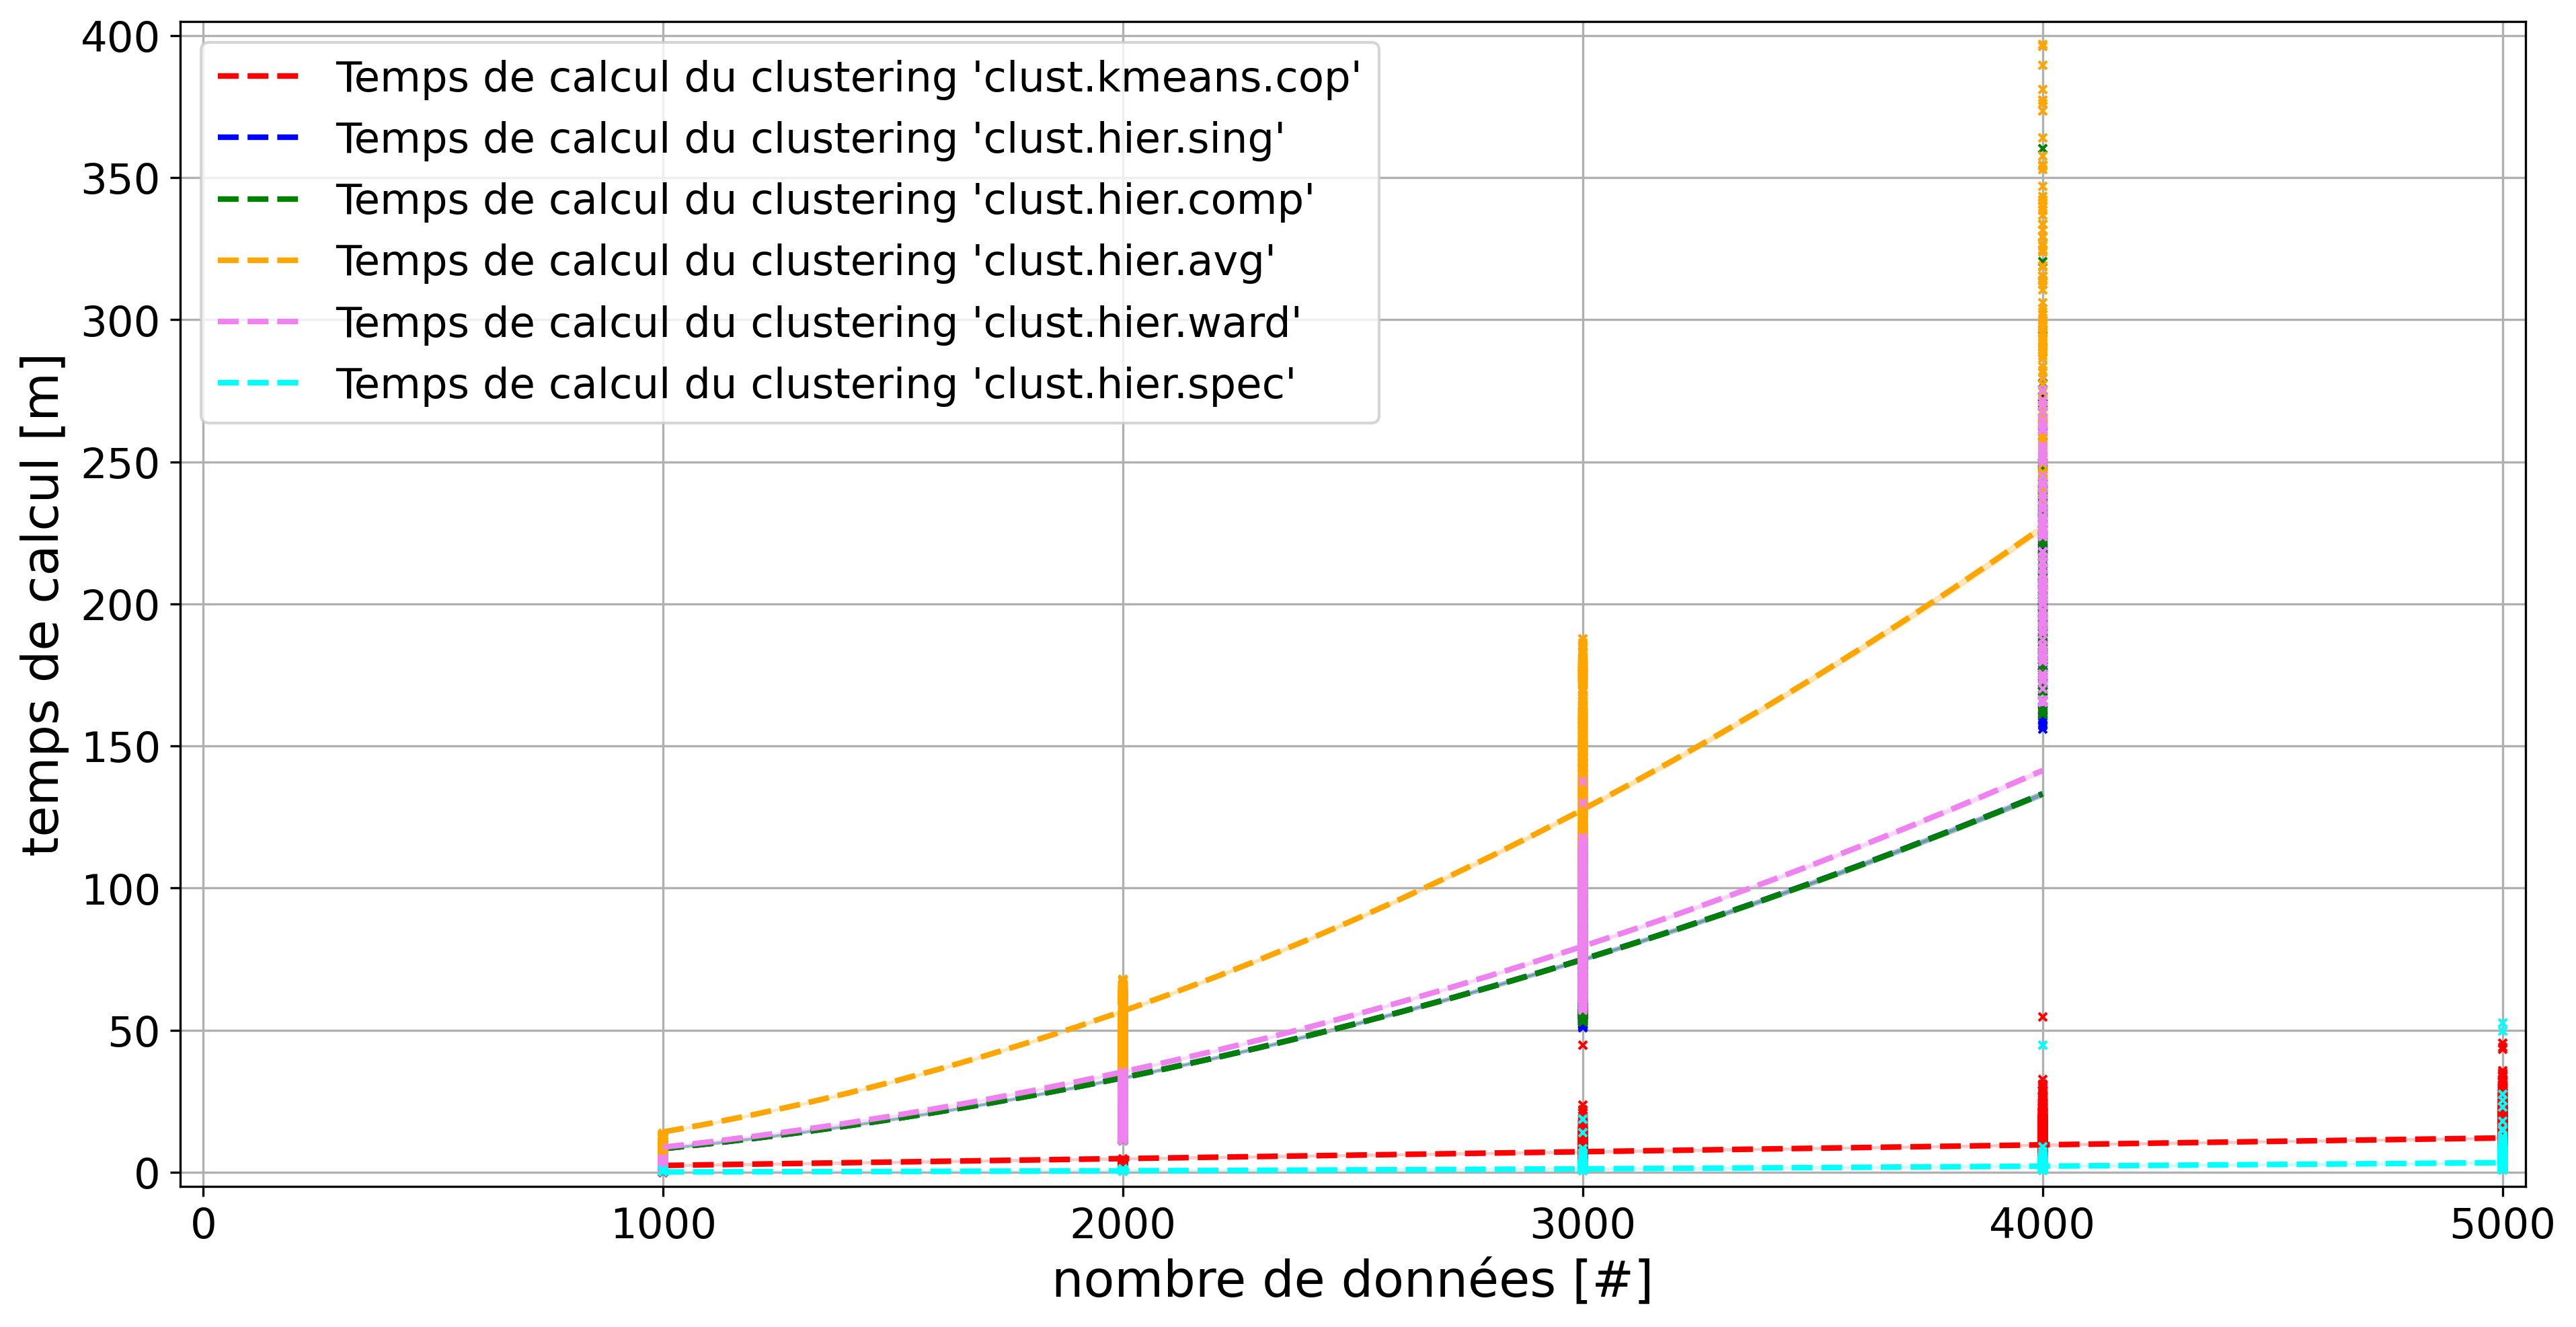
\includegraphics[width=0.8\textwidth]{figures/etude-temps-calcul-modelisation-3clust}
				\caption{Estimation du temps nécessaire (en secondes) pour effectuer une tâche de \textbf{clustering} en fonction du nombre de données à traiter.}
				\label{figure:4.3.2-ETUDE-COUTS-TEMPS-CALCUL-MODELISATION-CLUSTERING}
			\end{figure}
			
			%%% Sampling
			
			% Première analyse.
			En ce qui concerne la tâche d'\textbf{échantillonnage de contraintes}, une première analyse montre que les modélisations des quatre implémentations sont différentiables  (\texttt{p-valeur}: $<$ \texttt{$10^{-3}$}). Nous ferons donc une modélisation par algorithme.
			
			% Modélisation du temps de calcul (samp.rand.full).
			Pour les algorithmes de l'échantillonnage de contraintes \texttt{samp.rand.full}, l'analyse de la corrélation des facteurs avec les mesures de temps d'exécution indique qu'une modélisation minimale et suffisante peut être réalisée à partir du facteur $\texttt{dataset\_size}^{2}$ (\texttt{r}: $0.993$).
			Le second facteur le plus corrélé (mais non retenu) est l'interaction $\texttt{dataset\_size}^{2} \cdot previous\_nb\_clusters$ (\texttt{r}: $0.791$).
			Le modèle linéaire généralisé retenu (\texttt{R²}: $> 0.999$, \texttt{llf}: $-4.33 \cdot 10^{4}$, \texttt{llf\_null}: $-1.17 \cdot 10^{5}$) nous permet de déduire l'équation suivante\todo{ref complexité théorique algo en annexe} :
			%
			\begin{equation}
				time.samp.rand.full~(secondes)~
				\simeq~-0.48 + 8.47 \cdot 10^{-7} \cdot \texttt{dataset\_size}^{2}
			\end{equation}
			
			% Modélisation du temps de calcul (samp.rand.same).
			Pour les algorithmes de l'échantillonnage de contraintes \texttt{samp.rand.same}, l'analyse de la corrélation des facteurs avec les mesures de temps d'exécution indique qu'une modélisation minimale et suffisante peut être réalisée à partir du facteur $\texttt{dataset\_size}^{2}$ (\texttt{r}: $0.939$).
			Le second facteur le plus corrélé (mais non retenu) est l'interaction $\texttt{dataset\_size}^{2} \cdot algorithm\_nb\_constraints$ (\texttt{r}: $0.611$).
			Le modèle linéaire généralisé retenu (\texttt{R²}: $> 0.999$, \texttt{llf}: $-3.17 \cdot 10^{4}$, \texttt{llf\_null}: $-6.84 \cdot 10^{4}$) nous permet de déduire l'équation suivante\todo{ref complexité théorique algo en annexe} :
			%
			\begin{equation}
				time.samp.rand.same~(secondes)~
				\simeq~-0.14 + 1.92 \cdot 10^{-7} \cdot \texttt{dataset\_size}^{2}
			\end{equation}
			
			% Modélisation du temps de calcul (samp.farhtest.same).
			Pour les algorithmes de l'échantillonnage de contraintes \texttt{samp.farhtest.same}, l'analyse de la corrélation des facteurs avec les mesures de temps d'exécution indique qu'une modélisation minimale et suffisante peut être réalisée à partir du facteur $\texttt{dataset\_size}^{2}$ (\texttt{r}: $0.981$).
			Le second facteur le plus corrélé (mais non retenu) est l'interaction $\texttt{dataset\_size}^{2} \cdot previous\_nb\_clusters$ (\texttt{r}: $0.700$).
			Le modèle linéaire généralisé retenu (\texttt{R²}: $> 0.999$, \texttt{llf}: $-4.52 \cdot 10^{4}$, \texttt{llf\_null}: $-1.02 \cdot 10^{5}$) nous permet de déduire l'équation suivante\todo{ref complexité théorique algo en annexe} :
			%
			\begin{equation}
				time.samp.farhtest.same~(secondes)~
				\simeq~-0.23 + 5.32 \cdot 10^{-7} \cdot \texttt{dataset\_size}^{2}
			\end{equation}
			
			% Modélisation du temps de calcul (samp.closest.diff).
			Pour les algorithmes de l'échantillonnage de contraintes \texttt{samp.closest.diff}, l'analyse de la corrélation des facteurs avec les mesures de temps d'exécution indique qu'une modélisation minimale et suffisante peut être réalisée à partir du facteur $\texttt{dataset\_size}^{2}$ (\texttt{r}: $0.995$).
			Le second facteur le plus corrélé (mais non retenu) est l'interaction $\texttt{dataset\_size}^{2} \cdot previous\_nb\_clusters$ (\texttt{r}: $0.815$).
			Le modèle linéaire généralisé retenu (\texttt{R²}: $> 0.999$, \texttt{llf}: $-5.80 \cdot 10^{4}$, \texttt{llf\_null}: $-1.36 \cdot 10^{5}$) nous permet de déduire l'équation suivante\todo{ref complexité théorique algo en annexe} :
			%
			\begin{equation}
				time.samp.closest.diff~(secondes)~
				\simeq~-0.66 + 1.46 \cdot 10^{-6} \cdot \texttt{dataset\_size}^{2}
			\end{equation}
			
			% Affichage du temps de calcul.
			La figure~\ref{figure:4.3.2-ETUDE-COUTS-TEMPS-CALCUL-MODELISATION-SAMPLING} représente ces modélisations de temps de calcul des algorithmes d'échantillonnage en comparaison avec les mesures réalisées lors de l'expérience.
			\newline
			%
			\begin{figure}[!htb]
				\centering
				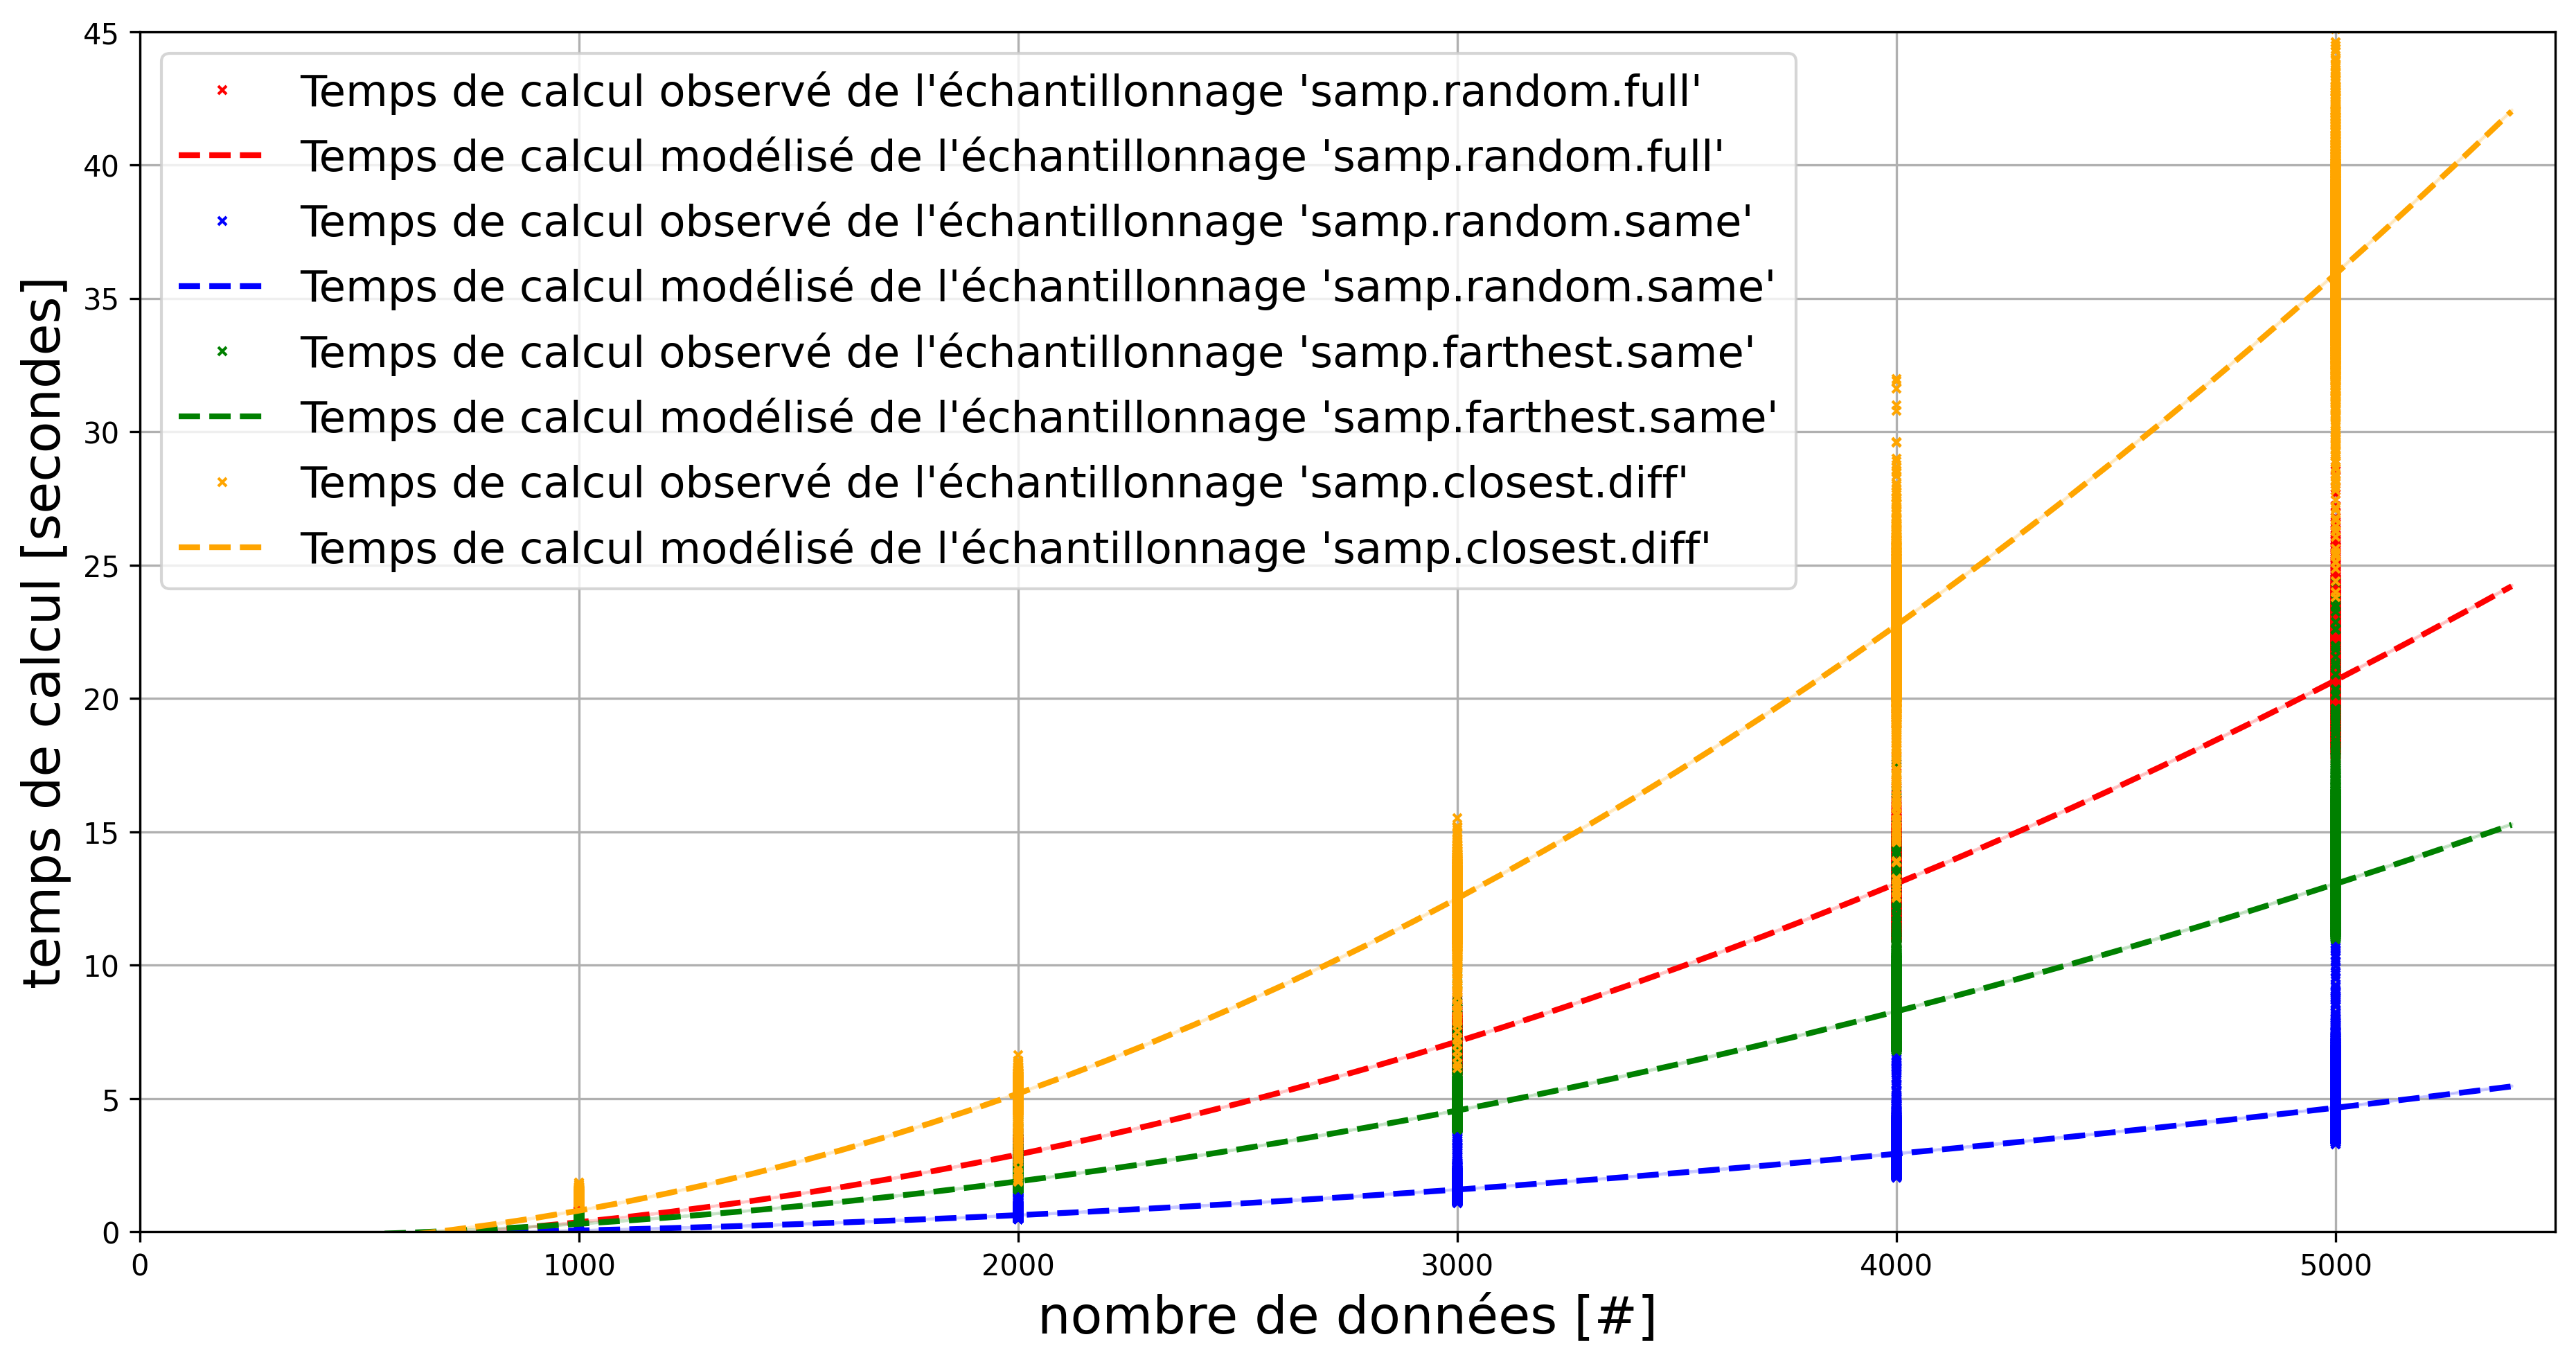
\includegraphics[width=0.8\textwidth]{figures/etude-temps-calcul-modelisation-4samp}
				\caption{Estimation du temps nécessaire (en secondes) pour effectuer une tâche d'\textbf{échantillonnage de contraintes} en fonction du nombre de données à traiter.}
				\label{figure:4.3.2-ETUDE-COUTS-TEMPS-CALCUL-MODELISATION-SAMPLING}
			\end{figure}

		%%% Discussion
		\subsubsection{Discussion}
		
			% Rappel de l'objectif : estimer le temps d'exécution.
			Dans cette étude, nous avons estimé le temps de calcul des différents algorithmes implémentés afin de confirmer le choix de paramétrage pour une convergence optimal (cf. hypothèse d'efficience en section~\ref{section:4.2-HYPOTHESE-EFFICIENCE}).
			Ces estimations ont été réalisées sur la base de plusieurs exécutions et fonction de divers contextes d'utilisation : nombre de données, nombre de contraintes annotées, nombre de contraintes à sélectionner, nombre de \textit{clusters} existant, nombre de \textit{clusters} à trouver.
			
			% Remarque générale : Dépend principalement du nombre de données.
			En premier lieu, on peut constater que les différentes modélisations dépendent majoritairement de la taille du jeu de données manipulé ($\texttt{dataset\_size}$ ou $\texttt{dataset\_size}^{2}$) avec un score de corrélation \texttt{r} avec le temps mesuré généralement supérieur à $0.9$ et des modèles \textit{GLM} avec des coefficients de détermination généralisé \texttt{R²} généralement proches de $0.999$.
			Bien que d'autres facteurs peuvent intervenir dans ces estimations (notamment les interactions doubles entre la taille du jeu de données et le nombre de \textit{clusters} ou le nombre de contraintes), ces derniers semblent avoir un impact négligeable sur le temps d'exécution.
			
			% Note: remarque sur le nombre de contraintes.
			\begin{leftBarAuthorOpinion}
				Certains paramétrages de la méthode du \textit{clustering} interactif semblent cependant avoir un temps de calcul décroissant au cours des itérations, mais nous n'avons cependant pas pu montrer de tendances globales significatives.
				Il est probable que l'ajout de contraintes judicieusement placées permettent à certains algorithmes de \textit{clustering} de s'exécuter plus rapidement, notamment lorsque ceux-ci exploitent les composants connexes du graphe de contraintes (cf. section~\ref{section:3.3.2-GESTION-DES-CONTRAINTES}). En effet, :
				\begin{itemize}
					\item les \textit{clustering} hiérarchiques s'initialisent autant de \textit{clusters} que de groupes de données liées entre elles par des contraintes \texttt{MUST-LINK} : or s'il y a plus de contraintes, alors les composants connexes sont davantage développés, donc il y a moins de \textit{clusters} à initialiser et donc moins d'époques de l'algorithme ;
					\item le \textit{clustering} KMeans (modèle COP) attire auprès d'un barycentre l'ensemble des données liées par un \texttt{MUST-LINK} : or s'il y a plus de contraintes, alors il y a des données attirées, donc les noyaux de \textit{clusters} peuvent se stabiliser plus rapidement.  
				\end{itemize}
				Toutefois, ces suppositions n'ont pas pu être démontrées, et certains contre-exemples tendent à conclure que ces comportements sont très dépendants du jeu de données manipulé et de l'ordre d'ajout des contraintes. Par exemple :
				\begin{itemize}
					\item l'ajout d'un trop grand nombre de contraintes \texttt{CANNOT-LINK} peut engendrer un surplus de vérification pour estimer quelles formations de \textit{clusters} sont autorisées sans violer de contraintes ;
					\item l'algorithme KMeans (modèle COP) peut osciller autour de plusieurs noyaux de \textit{clusters} instables si les contraintes violent trop la similarité intrinsèque des données.
				\end{itemize}
			\end{leftBarAuthorOpinion}
			
			% Cas du clustering.
			En ce qui concerne la tâche de \textit{clustering}, on note des différences significatives dans les temps d'exécution des divers algorithmes implémentés.
			En effet, l'algorithme KMeans (modèle COP) est nettement plus rapide (complexité en $ \mathcal{O}(\texttt{dataset\_size}) $, nécessitant quelques dizaines de minutes pour $5~000$ données) que les implémentations du \textit{clustering} hiérarchique (complexité en $ \mathcal{O}(\texttt{dataset\_size}^{2}) $, nécessitant plusieurs heures pour $5~000$ données).
			Cette différence, visible en figure~\ref{figure:4.3.2-ETUDE-COUTS-TEMPS-CALCUL-MODELISATION-CLUSTERING}, a un réel impact sur l'expérience utilisateur de l'opérateur.
			En effet, bien qu'il soit théoriquement plus efficient pour atteindre une annotation suffisante (cf. hypothèse d'efficience en section~\ref{section:4.2-HYPOTHESE-EFFICIENCE}), l'usage d'un \textit{clustering} hiérarchique imposerait de longs temps d'attente à l'opérateur, interdisant des interactions rapides avec la machines.
			Or l'intérêt principal de notre méthodologie d'annotation à l'aide du \textit{clustering} interactif repose sur ces interactions homme-machine via l'ajout régulier de contraintes pertinentes (cf. hypothèse d'efficacité en section~\ref{section:4.1-HYPOTHESE-EFFICACITE}).
			Nous décidons donc d'exclure l'usage des algorithmes de \textit{clustering} hiérarchique au profit du \textit{clustering} KMeans (modèle COP).
			
			% Note: Cas du projet étudiant avec TPS.
			\begin{leftBarInformation}
				Dans le cadre du projet étudiant avec l'école Télécom Physique Strasbourg visant à implémenter d'autres algorithmes de \textit{clustering} sous contraintes, un résonnement similaire a été utilisé pour filtrer les algorithmes. Ainsi, l'implémentation de KMeans (modèle MPC) a été exclu (complexité en $ \mathcal{O}(\texttt{dataset\_size}^{3}) $) et l'implémentation de la propagation par affinité écarte la gestion des contraintes \texttt{CANNOT-LINK} pour avoir un temps d'exécution comparable au \textit{clustering} KMeans (modèle COP). L'algorithme DBScan (modèle C-DBScan) est quand à lui un rival possible avec une complexité théorique en $ \mathcal{O}(\texttt{dataset\_size}) $.
			\end{leftBarInformation}
			
			% Cas du prétraitement + vectorisation + échantillonage.
			En ce qui concerne les tâches de prétraitements (figure~\ref{figure:4.3.2-ETUDE-COUTS-TEMPS-CALCUL-MODELISATION-PREPROCESSING}), de vectorisation (figure~\ref{figure:4.3.2-ETUDE-COUTS-TEMPS-CALCUL-MODELISATION-VECTORIZATION}), et d'échantillonnage de contraintes (cf. figure~\ref{figure:4.3.2-ETUDE-COUTS-TEMPS-CALCUL-MODELISATION-SAMPLING}) ont des complexités presque négligeables au regard des temps d'exécution du \textit{clustering} (pour $5~000$ données : environ $60$ secondes contre près de $800$ secondes pour \texttt{clust.kmeans.cop} et près de $15~000$ secondes pour \texttt{clust.hier.sing}).
			Nous maintenons donc les paramétrages obtenus pour ces tâches en section~\ref{section:4.2-HYPOTHESE-EFFICIENCE} sans analyses complémentaires et bornons l'ensemble des ces temps de calcul par un temps constant de $60$ secondes.
			
			% Conclusion.
			Pour conclure, dans l'optique d'atteindre de manière efficiente $90$\% de \texttt{v-measure}
			\footnote{$90$\% de \texttt{v-measure}: cas d'une annotation dite partielle, dont le paramétrage le plus efficient est constitué du prétraitement simple (\texttt{prep.simple}), de la vectorisation TF-IDF (\texttt{vect.tfidf}), du clustering hiérarchique à lien moyen (\texttt{clust.hier.avg}) et de l'échantillonnage des données les plus proches dans des clusters différents (\texttt{sampl.closest.diff}}
			avec un coût global minimal, nous retenons l'usage du \textbf{paramétrage favori} constitué du prétraitement simple (\texttt{prep.simple}), de la vectorisation TF-IDF (\texttt{vect.tfidf}), du clustering KMeans avec modèle COP (\texttt{clust.kmeans.cop}) et de l'échantillonnage des données les plus proches dans des clusters différents (\texttt{sampl.closest.diff}).
			On estime le temps d'exécution de ce paramétrage avec l'équation suivante\footnote{Temps du paramétrage favori : environ $30$ secondes pour $1~000$ données ; environ $15$ minutes pour $5~000$ données.} :
			%
			\begin{equation}
				time.parametrage.favori~(secondes)~
				\simeq~-180 + 2.11 \cdot 10^{-1} \cdot \texttt{dataset\_size}
			\end{equation}
	
	%%%
	%%% Subsection 4.3.3: Étude du nombre de contraintes nécessaires à la convergence vers une vérité terrain pré-établie en fonction de la taille du jeu de données 
	%%%
	\subsection{Étude du nombre de contraintes nécessaires à la convergence vers une vérité terrain pré-établie en fonction de la taille du jeu de données}
	\label{section:4.3.3-ETUDE-COUT-NOMBRE-CONTRAINTES}
	
		%%% Protocole expérimental.
		\subsubsection{Protocole expérimental}
			
			% Transition.
			Avec les deux précédentes études, nous sommes capable d'estimer le temps nécessaire à un expert pour annoter des contraintes et le temps nécessaire à la machine pour proposer un nouveau \textit{clustering} adapté aux suggestions de l'expert.
			Pour poursuivre nos études et pouvoir estimer le coût total d'un projet d'annotation, il nous reste à estimer le nombre total de contraintes à devoir renseigner en fonction de la taille du jeu de données.
			
			% Objectif de l'expérience.
			Pour cela, nous allons simuler la création de cette base d'apprentissage en adaptant le protocole utilisé lors de notre étude d'efficacité (cf. section~\ref{section:4.1.1-ETUDE-CONVERGENCE}) :
			nous emploierons notre méthode de \textit{clustering} interactif avec notre \textbf{paramétrage favori}
			\footnote{Paramétrage favori (atteindre $90$\% de \texttt{v-measure} avec un coût minimal): prétraitement simple (\texttt{prep.simple}), vectorisation TF-IDF (\texttt{vect.tfidf}), clustering KMeans avec modèle COP (\texttt{clust.kmeans.cop}) et échantillonnage des données les plus proches dans des clusters différents (\texttt{sampl.closest.diff})}
			sur des jeux de données de différentes tailles et mesurerons le nombre de contraintes nécessaires pour converger vers la vérité terrain.
			
			% Axiome et Remarque.
			\begin{leftBarWarning}
				Dans le cadre de cette étude, nous supposons que l'expert métier connaît parfaitement le domaine traité dans ce jeu de données, et qu'il est capable de caractériser sans ambiguïté la similitude entre deux données issues de cet ensemble.
				De plus, pour utiliser des jeux de données de tailles différentes tout en maîtrisant leur contenu, nous avons dupliqués aléatoirement des données issues de deux jeux de référence en générant des fautes de frappes.
				Pour cette étude, nous faisons l'hypothèse que cela n'a pas d'impact majeur sur le nombre de contraintes nécessaires pour converger vers la vérité terrain.
			\end{leftBarWarning}
			
			% Pseudo-code.
			Pour résumer le protocole expérimental que nous décrivons ci-dessous, vous pouvez vous référer au pseudo-code décrit dans Alg.~\ref{algorithm:4.3.3-ETUDE-COUT-NOMBRE-CONTRAINTES-PROTOCOLE}.
			%
			\begin{algorithm}[!htb]
				\begin{algorithmic}[1]
					\Require jeux de données annotés (vérité terrain) de tailles différentes
					\ForAll{jeux de données à tester}
						\State \textbf{initialisation (données)}: récupérer ou générer les données et la vérité terrain
						\State \textbf{initialisation (contraintes)}: créer une liste vide de contraintes
						\State \textbf{prétraitement}: supprimer le bruit dans les données avec \texttt{prep.simple}
						\State \textbf{vectorisation}: transformer les données en vecteurs avec \texttt{vect.tfidf}
						\State \textbf{clustering initial}: regrouper les données par similarité avec \texttt{clust.kmeans.cop}
						\State \textbf{évaluation}: estimer l'équivalence entre le clustering obtenu et la vérité terrain
						\Repeat
							\State \textbf{échantillonnage}: sélectionner de nouvelles contraintes à annoter
							\State \textbf{simulation d'annotation}: ajouter des contraintes avec \texttt{samp.closest.diff}
							\State \textbf{clustering}: regrouper les données par similarité avec \texttt{clust.kmeans.cop}
							\State \textbf{évaluation}: estimer l'équivalence entre le clustering obtenu et la vérité terrain
						\Until{annotation de toutes les contraintes possibles}
					\EndFor						
					\State \textbf{analyse}: entraîner un modèle linéaire généralisé du nombre de contraintes nécessaires à la convergence
					\Ensure modélisation du nombre de contraintes nécessaires pour un jeu de données
				\end{algorithmic}
				\caption{Description en pseudo-code du protocole expérimental de l'étude du nombre de contraintes nécessaires pour converger vers une vérité terrain pré-établie avec notre paramétrage favori du \textit{clustering} interactif.}
				\label{algorithm:4.3.3-ETUDE-COUT-NOMBRE-CONTRAINTES-PROTOCOLE}
			\end{algorithm}
			
			% Description des jeux de données.
			Pour cette étude, nous utilisons comme références les jeux de données \textbf{TODO:JDD}\todo{TODO: reference dataset bank card} et \textbf{TODO:JDD}\todo{TODO: reference dataset mlsum}.
			La taille des jeux de données générée, noté $\texttt{dataset\_size}$, varie entre $1~000$ à $5~000$ par pas de $250$, et chaque taille de jeu est générée $3$ fois pour contrer les aléas statistiques de création.
			Il y a donc $51$ variations de chaque jeu de références, soit $102$ jeux utilisés de tailles différentes.
			
			% Description des tentatives de la méthode.
			Sur chacun de ces jeux générés, une tentative complète
			\footnote{Tentative complète : itérations d'échantillonnage, d'annotation et de \textit{clustering} jusqu'à annotation de toutes les contraintes possibles.}
			de la méthode du \textit{clustering} interactif utilisant notre paramétrage favori est exécuté, et chaque tentative est répétée $5$ fois pour contrer les aléas statistiques des exécutions.
			Il y a donc $510$ tentatives de \textit{clustering} interactif réalisées.
			
			% Description de l'évaluation.
			Pour chacune de ces tentatives, nous nous intéresserons au nombre de contraintes nécessaires pour atteindre le seuil d'annotation partielle (caractérisé par $90$\% de \texttt{v-measure} entre la vérité terrain et la segmentation des données obtenue), et nous entraînerons un modèle linéaire généralisé (\textit{GLM}) pour modéliser le nombre de contraintes requis en fonction de la taille du jeu de données.
			Ce modèle sera caractérisé par le coefficient de détermination généralisé \texttt{R²} de \textit{Cox et Snel}, la log-vraisemblance \texttt{llf} et la log-vraisemblance \texttt{llf\_null} du modèle \textit{null}.
			Pour finir, nous discuterons des valeurs des coefficients obtenus sur l'impact du nombre d'itérations de la méthode à prévoir.

			% Référence scripts.
			\begin{leftBarInformation}
				Ces analyses sont réalisées en Python à l'aide de la librairie \texttt{statsmodels} (\cite{seabold:2010}).
				Les scripts de l'expérience (\textit{notebooks} Python) sont disponibles dans un dossier dédié de~\cite{schild:cognitivefactory-interactive-clustering-comparative-study:2021}.
			\end{leftBarInformation}

		%%% Résultats
		\subsubsection{Résultats obtenus}
		
			\todo[inline]{figure évolution nb contraintes par rapport à la taille du JDD}
			\todo[inline]{équation évolution nb contraintes par rapport à la taille du JDD}

		%%% Discussion
		\subsubsection{Discussion}
		
			\todo[inline]{A REDIGER : linéaire ? diffères des deux JDD ?}
	
	%%%
	%%% Subsection 4.3.4: Estimation du temps total d'un projet d'annotation en combinant les précédentes études de coûts
	%%%
	\subsection{Estimation du temps total d'un projet d'annotation en combinant les précédentes études de coûts}
	\label{section:4.3.4-ETUDE-COUTS-TOTAL}

		%%% Résultats
		\subsubsection{Résultats obtenus}

		%%% Discussion
		\subsubsection{Discussion}